
\chapter{变化检测任务与实验方法介绍}
遥感影像变化检测(Remote Sensing Change Detection, RSCD)是遥感技术中的一个重要应用,旨在通过对比两幅或多幅在不同时间拍摄的遥感影像,识别出地表的变化区域~\cite{YGXB202407012}。随着遥感技术的进步和深度学习技术的应用,变化检测任务已经逐渐从传统的像素差异法、图像配准方法,发展为基于深度神经网络的方法。这些方法能够更准确地从遥感影像中提取特征,识别变化区域,尤其是在复杂背景和微小变化的情况下。

\section{变化检测任务介绍}

变化检测任务的核心目标是识别在不同时间点拍摄的两幅或多幅遥感影像之间的差异。这一任务对于环境监测、灾害评估、城市扩展检测、资源管理等多个领域具有重要意义。传统的变化检测方法主要依赖于像素级别的差异分析,而随着深度学习技术的引入,基于深度神经网络的变化检测方法通过自动学习多层次特征和复杂模式,显著提高了变化检测的精度和鲁棒性。

在目前普遍应用的基于深度学习的变化检测任务中,通常涉及到以下几个关键任务:

\textbf{双时相影像配准}:由于双时相的遥感影像在获取过程中可能存在拍摄时间、传感器类型及成像角度等方面的差异,图像配准成为变化检测的前提~\cite{WHCH202405001}。高精度的配准能够保证双时相影像在空间位置上的一致性,从而为后续的差异分析和变化识别提供可靠基础。同时,双时相影像在空间位置上的一致性,也是普遍的全监督变化检测任务能够成功进行的前提。配准方法通常包括基于特征点的配准、基于图像块的配准以及基于深度学习的配准等~\cite{YGXB202406011}。

\textbf{双时相影像差异特征分析}:在遥感影像变化检测任务中,双时相影像差异特征分析是至关重要的一步~\cite{CHXB202207001}。传统的差异计算方法通常依赖于像素级别的对比,如直接相减或计算变化指数。然而,随着深度学习技术的引入,基于神经网络的方法可以自动学习影像中的深层次特征,从而更准确地捕捉图像中的微小变化。在深度学习框架下,差异特征计算主要依赖于模型通过训练学习到的高级视觉特征。通过卷积神经网络(CNN)或其他深度学习模型提取双时相影像的多层次特征后,网络能够学习到不同时间点影像之间的差异性~\cite{chen_spatial-temporal_2020,lin_transition_2023,shi_deeply_2022}。这种方法不仅能够识别明显的变化区域,还能够识别由于地形变化、光照变化等因素导致的微小变化。

\textbf{变化区域识别与分类}:在变化区域的分类过程中,深度神经网络能够通过对比不同时间点的影像特征,自动学习变化与不变化区域的区分方法。对于不同的变化类型(如建筑物、新建道路、植被变化等),模型可以进一步将变化区域进行细化分类。通常,变化检测任务在变化区域的分类上与语义分割任务类似,均是利用神经网络进行像素级的分类任务。这些网络结构通过编码器-解码器的架构,可以在编码阶段提取高层次的特征表示,并通过解码阶段逐步恢复图像的空间分辨率,从而实现精细的像素级预测。然而,与侧重于单幅影像空间语义理解的语义分割不同,变化检测的核心目标是识别目标语义类别是否发生变化,而非仅仅是识别静态的语义类别本身,这对其特征提取和差异判别能力提出了更高的要求。在变化检测任务中,网络通过学习图像的时空特征差异,能够自动识别出哪些区域发生了变化,并将变化区域与不变区域区分开来。 

除此之外,为了系统性地评测和比较不同变化检测算法在上述关键环节中的性能,并推动算法向更高精度、更强鲁棒性的方向发展,相关研究人员构建了一系列公开的变化检测任务基准数据集。这些数据集的多样性和挑战性,为算法的有效性验证和泛化能力分析提供了重要的实验基础。

\section{常用的变化检测数据集介绍}
遥感影像变化检测的研究依赖于大量的实验数据集。为了证明本文本在变化检测任务的研究的广泛性和深刻性,本文选用了多种不同数据偏重的变化检测数据集来进行实验。这些数据集涵盖了不同的地理区域、变化类型以及影像质量,从而确保实验结果的广泛适用性。数据集包括了城市区域、农业区域、自然环境、海洋周边区域等多种场景,涉及建筑物变化、农田变化、水体变化等多种变化类型。这些数据集的多样性使得能够从多个角度对变化检测算法进行深入分析,探讨其在不同场景下的表现和局限性。具体而言,这些数据集分别在变化尺度、目标密度、背景复杂性、以及由季节和光照引起的伪变化等方面构成了不同的挑战,从而能够全面地检验变化检测算法的综合性能。

\subsection{针对建筑物区域的变化检测数据集}
\subsubsection{LEVIR-CD与LEVIR-CD+数据集}
LEVIR-CD~\cite{chen_spatial-temporal_2020}是一个大规模的遥感建筑变化检测数据集,旨在为变化检测(CD)算法,特别是基于深度学习的算法,提供一个新的评估基准。该数据集包含637对高分辨率(0.5m/像素)的Google Earth图像块,其中445对训练样本,64对验证样本,128对测试样本。每个图像块的大小为1024 × 1024像素,图像覆盖的时间跨度为5至14年,具有显著的土地利用变化,特别是建筑增长。如图~\ref{fig:levir_cd}所示,LEVIR-CD数据集重点关注与建筑物相关的变化,包括建筑物增长(从土壤、草地或建设中的建筑转变为新的建筑区域)和建筑物的减少。每对图像都由遥感图像解说专家进行二进制标签注释,最终提供了31,333个单独的建筑变化实例。数据集的地理空间分布包括美国德克萨斯州的多个城市,图像采集时间从2002年到2018年不等。由于不同区域的图像拍摄时间存在差异,该数据集引入了季节变化和光照变化的影响,这将有助于开发能够缓解这些不相关变化对实际变化影响的有效方法。LEVIR-CD数据集的构建提供了一个高质量的基准,具有丰富的建筑物变化实例,是建筑物变化检测任务中最常用的开源数据集之一。如图~\ref{fig:levir_cd_plus}所示, LEVIR-CD+~\cite{chen_spatial-temporal_2020}数据集是LEVIR-CD的扩展版本,包含985对遥感图像,其中637对属于训练数据集,其余的用于测试。

\begin{figure}[!htbp]
  \centering
  \includegraphics[width=0.75\textwidth]{paper_figures/变化检测任务与实验方法介绍/levir_cd.png}
  \caption{LEVIR-CD 数据集展示.}
  \label{fig:levir_cd}
\end{figure}

\begin{figure}[!htbp]
  \centering
  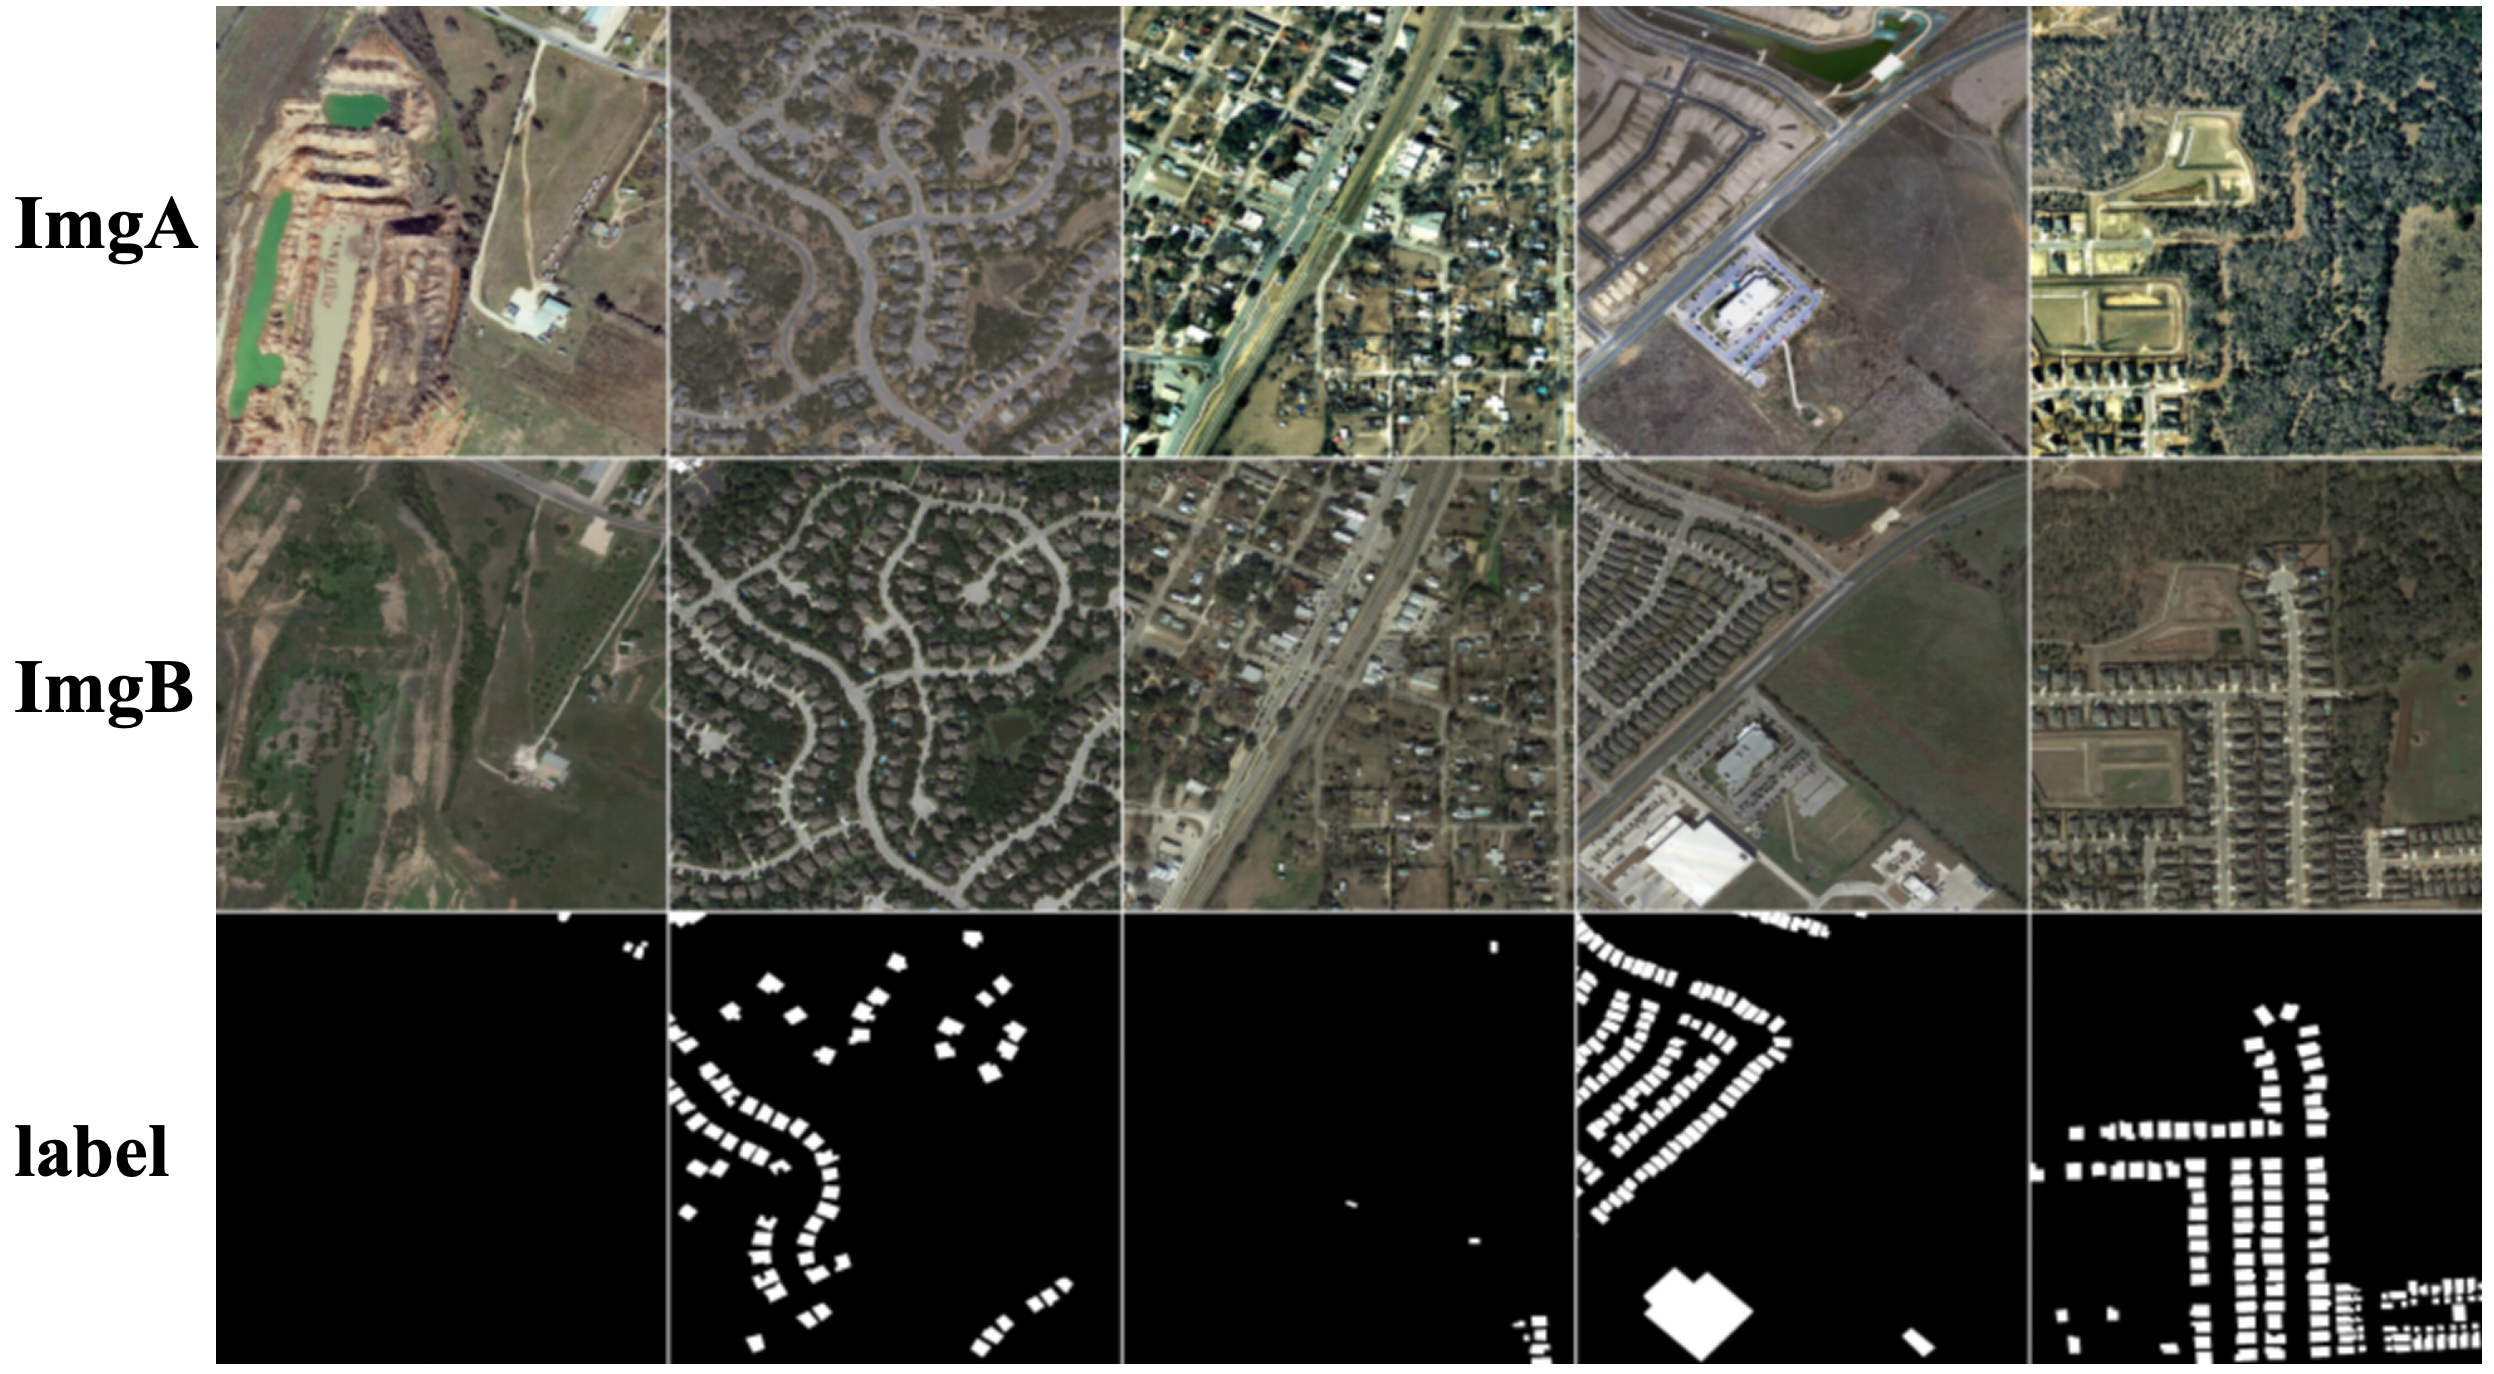
\includegraphics[width=0.75\textwidth]{paper_figures/变化检测任务与实验方法介绍/levir_cd_plus.png}
  \caption{LEVIR-CD+ 数据集展示.}
  \label{fig:levir_cd_plus}
\end{figure}

\subsubsection{S2Looking数据集}
S2Looking数据集~\cite{Shen2021S2LookingAS}是为推动建筑物变化检测研究而创建的,提供了一个新的、更具挑战性的资源。与LEVIR-CD+数据集相比,S2Looking扩展了数据集的规模,涵盖了农村地区的侧视遥感图像。由于其特殊的图像角度,S2Looking数据集所面临的变化检测问题与传统的基于Google Earth图像的数据集有所不同。数据集中包含了大量的建筑物增长和衰退的变化,但由于农村地区建筑物更新的稀疏性,这些变化的检测更具挑战性,如图~\ref{fig:s2looking}所示。

S2Looking数据集的一个显著特点是建筑变化实例的稀疏性。农村地区大多覆盖农田和森林,建筑物较为稀少,而城市地区则是建筑物密集、不断变化的区域。S2Looking中的变化实例数量较少,平均为13.184个,而LEVIR-CD中的变化实例为49.188个。这使得在进行建筑特征提取时,网络需要更好地适应稀疏数据和复杂背景。此外,S2Looking数据集采用侧视遥感图像,建筑物的影像是由卫星从不同的角度拍摄并投影成二维图像,这使得变化检测模型需要能够识别从不同角度拍摄的同一建筑物并检测其变化。由于农村地区季节性变化和与建筑更新无关的土地覆盖变化更加明显,S2Looking数据集面临着更为复杂的环境。农田的季节性变化和不同作物的覆盖使得土地在遥感图像中呈现不同的外观。因此,适用于此数据集的变化检测模型必须能够区分建筑变化与这些无关变化,以减少误检。

\begin{figure}[!htbp]
  \centering
  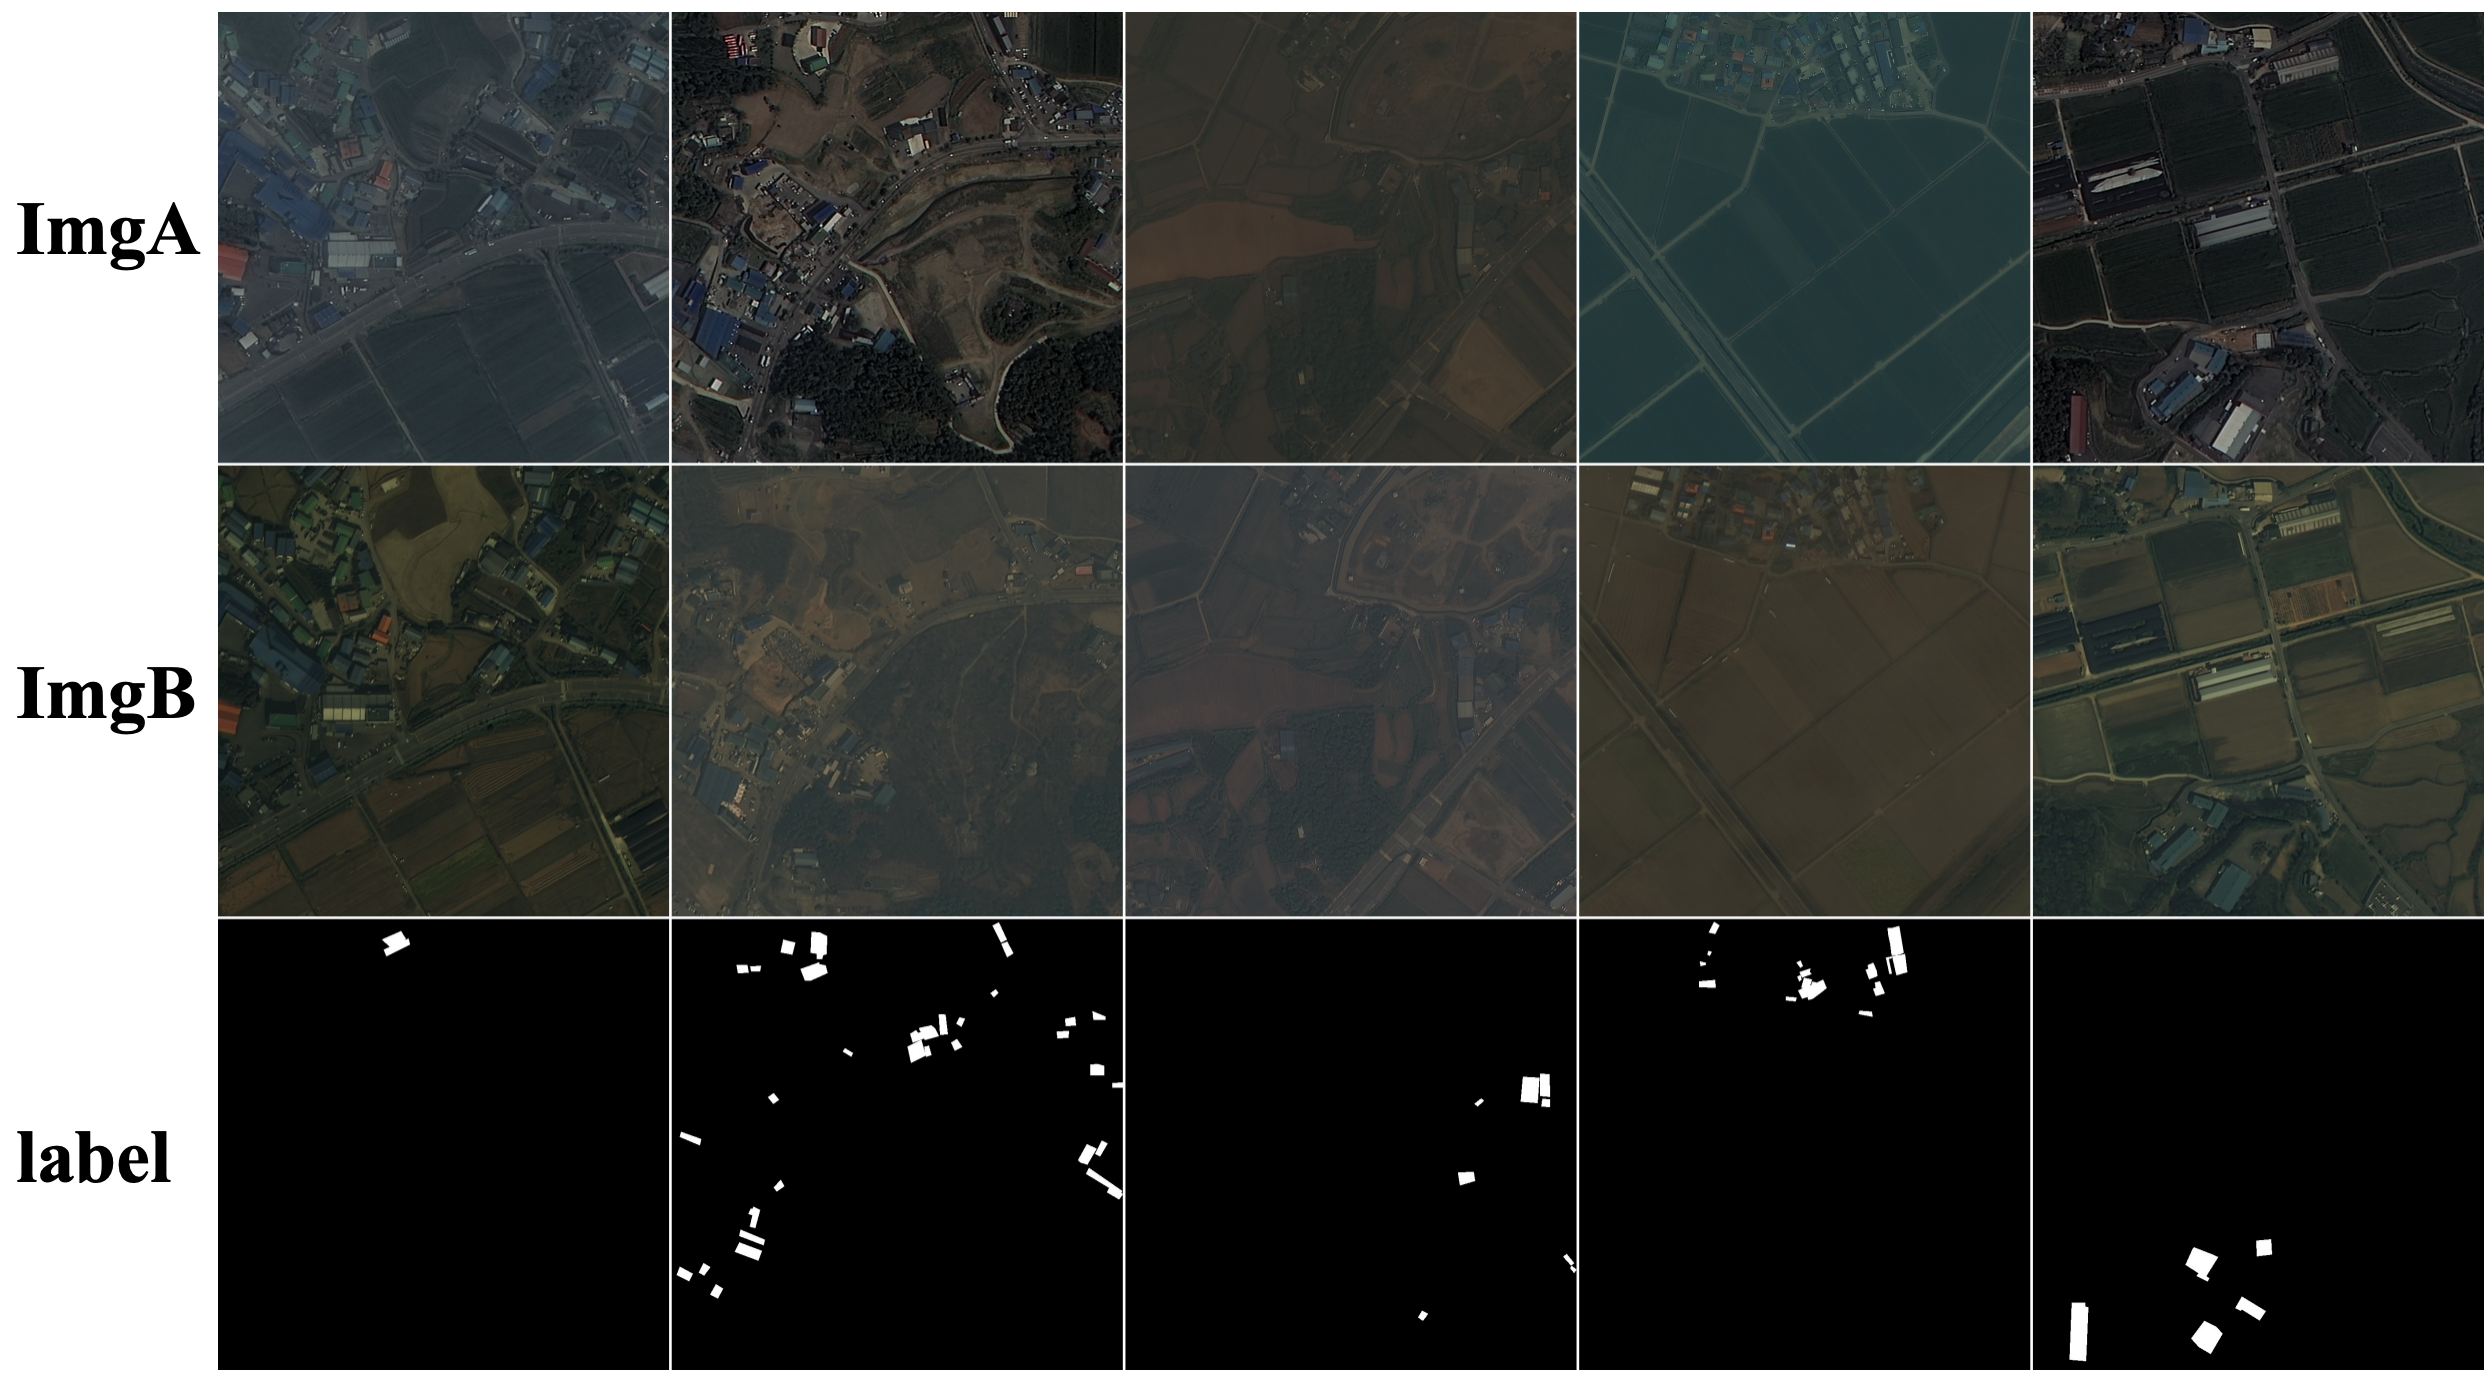
\includegraphics[width=0.75\textwidth]{paper_figures/变化检测任务与实验方法介绍/s2looking.png}
  \caption{S2Looking 数据集展示.}
  \label{fig:s2looking}
\end{figure}


\subsubsection{WHUCD数据集}
WHU建筑物数据集~\cite{Ji2019FullyCN}是一个由航拍图像和卫星图像构成的建筑物样本数据集,旨在为建筑物提取和变化检测研究提供重要的数据支持。该数据集包含超过220,000座独立建筑物,其中航拍数据集来自新西兰基督城,图像的空间分辨率为0.075米,覆盖面积达到450平方公里。在WHUCD的实验中,对原始的大尺寸影像进行裁剪,按照$256 \times 256$大小进行切分,如图~\ref{fig:whucd}所示。最终按照8:1:1的比例,得到6096张训练集图片,762张验证集图片,以及762张测试集图片。


\begin{figure}[!htbp]
  \centering
  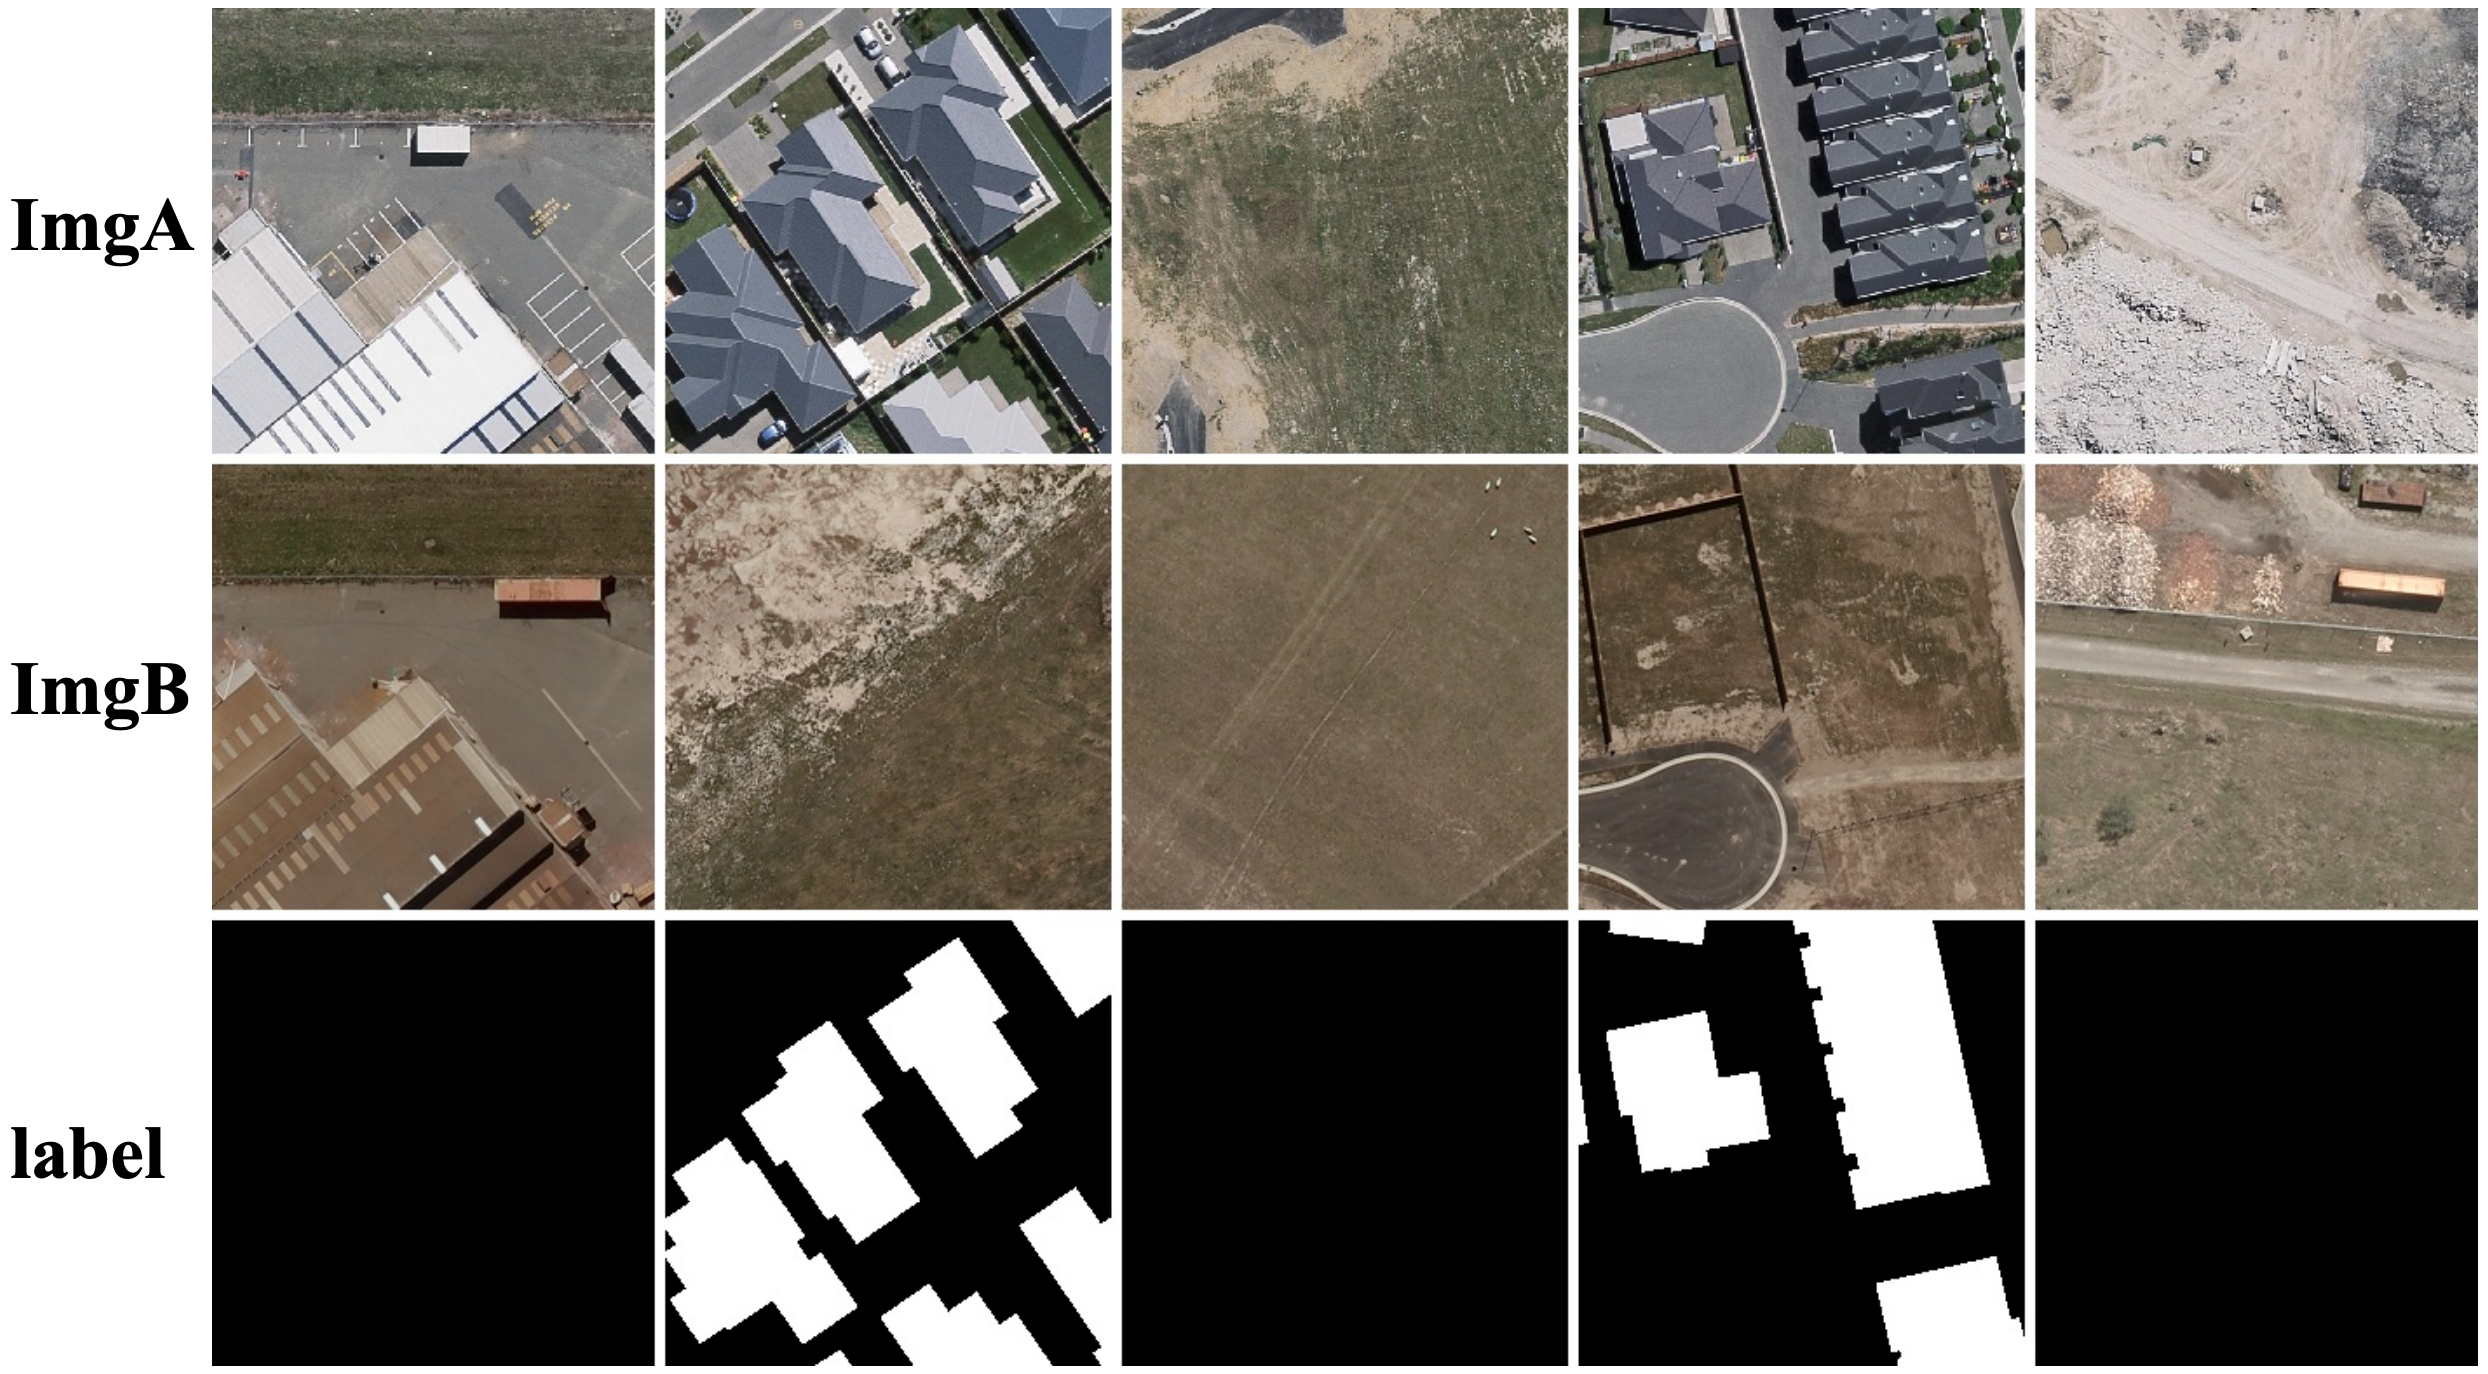
\includegraphics[width=0.75\textwidth]{paper_figures/变化检测任务与实验方法介绍/whucd.png}
  \caption{WHUCD 数据集展示.}
  \label{fig:whucd}
\end{figure}

\subsection{针对农田区域的变化检测数据集}
\subsubsection{CLCD数据集}
CLCD数据集~\cite{Liu2022ACN}由600对农田变化样本图像组成,其中320对用于训练,120对用于验证,120对用于测试。CLCD中的双时相图像分别由高分二号卫星于2017年和2019年在中国广东省采集,空间分辨率范围为0.5米至2米。每组样本由两张512 × 512的图像和对应的农田变化二进制标签组成。如图~\ref{fig:clcd}所示,CLCD中标注的主要变化类型为耕地类型的变化,包括耕地的开垦、休耕和复垦等。

\begin{figure}[!htbp]
  \centering
  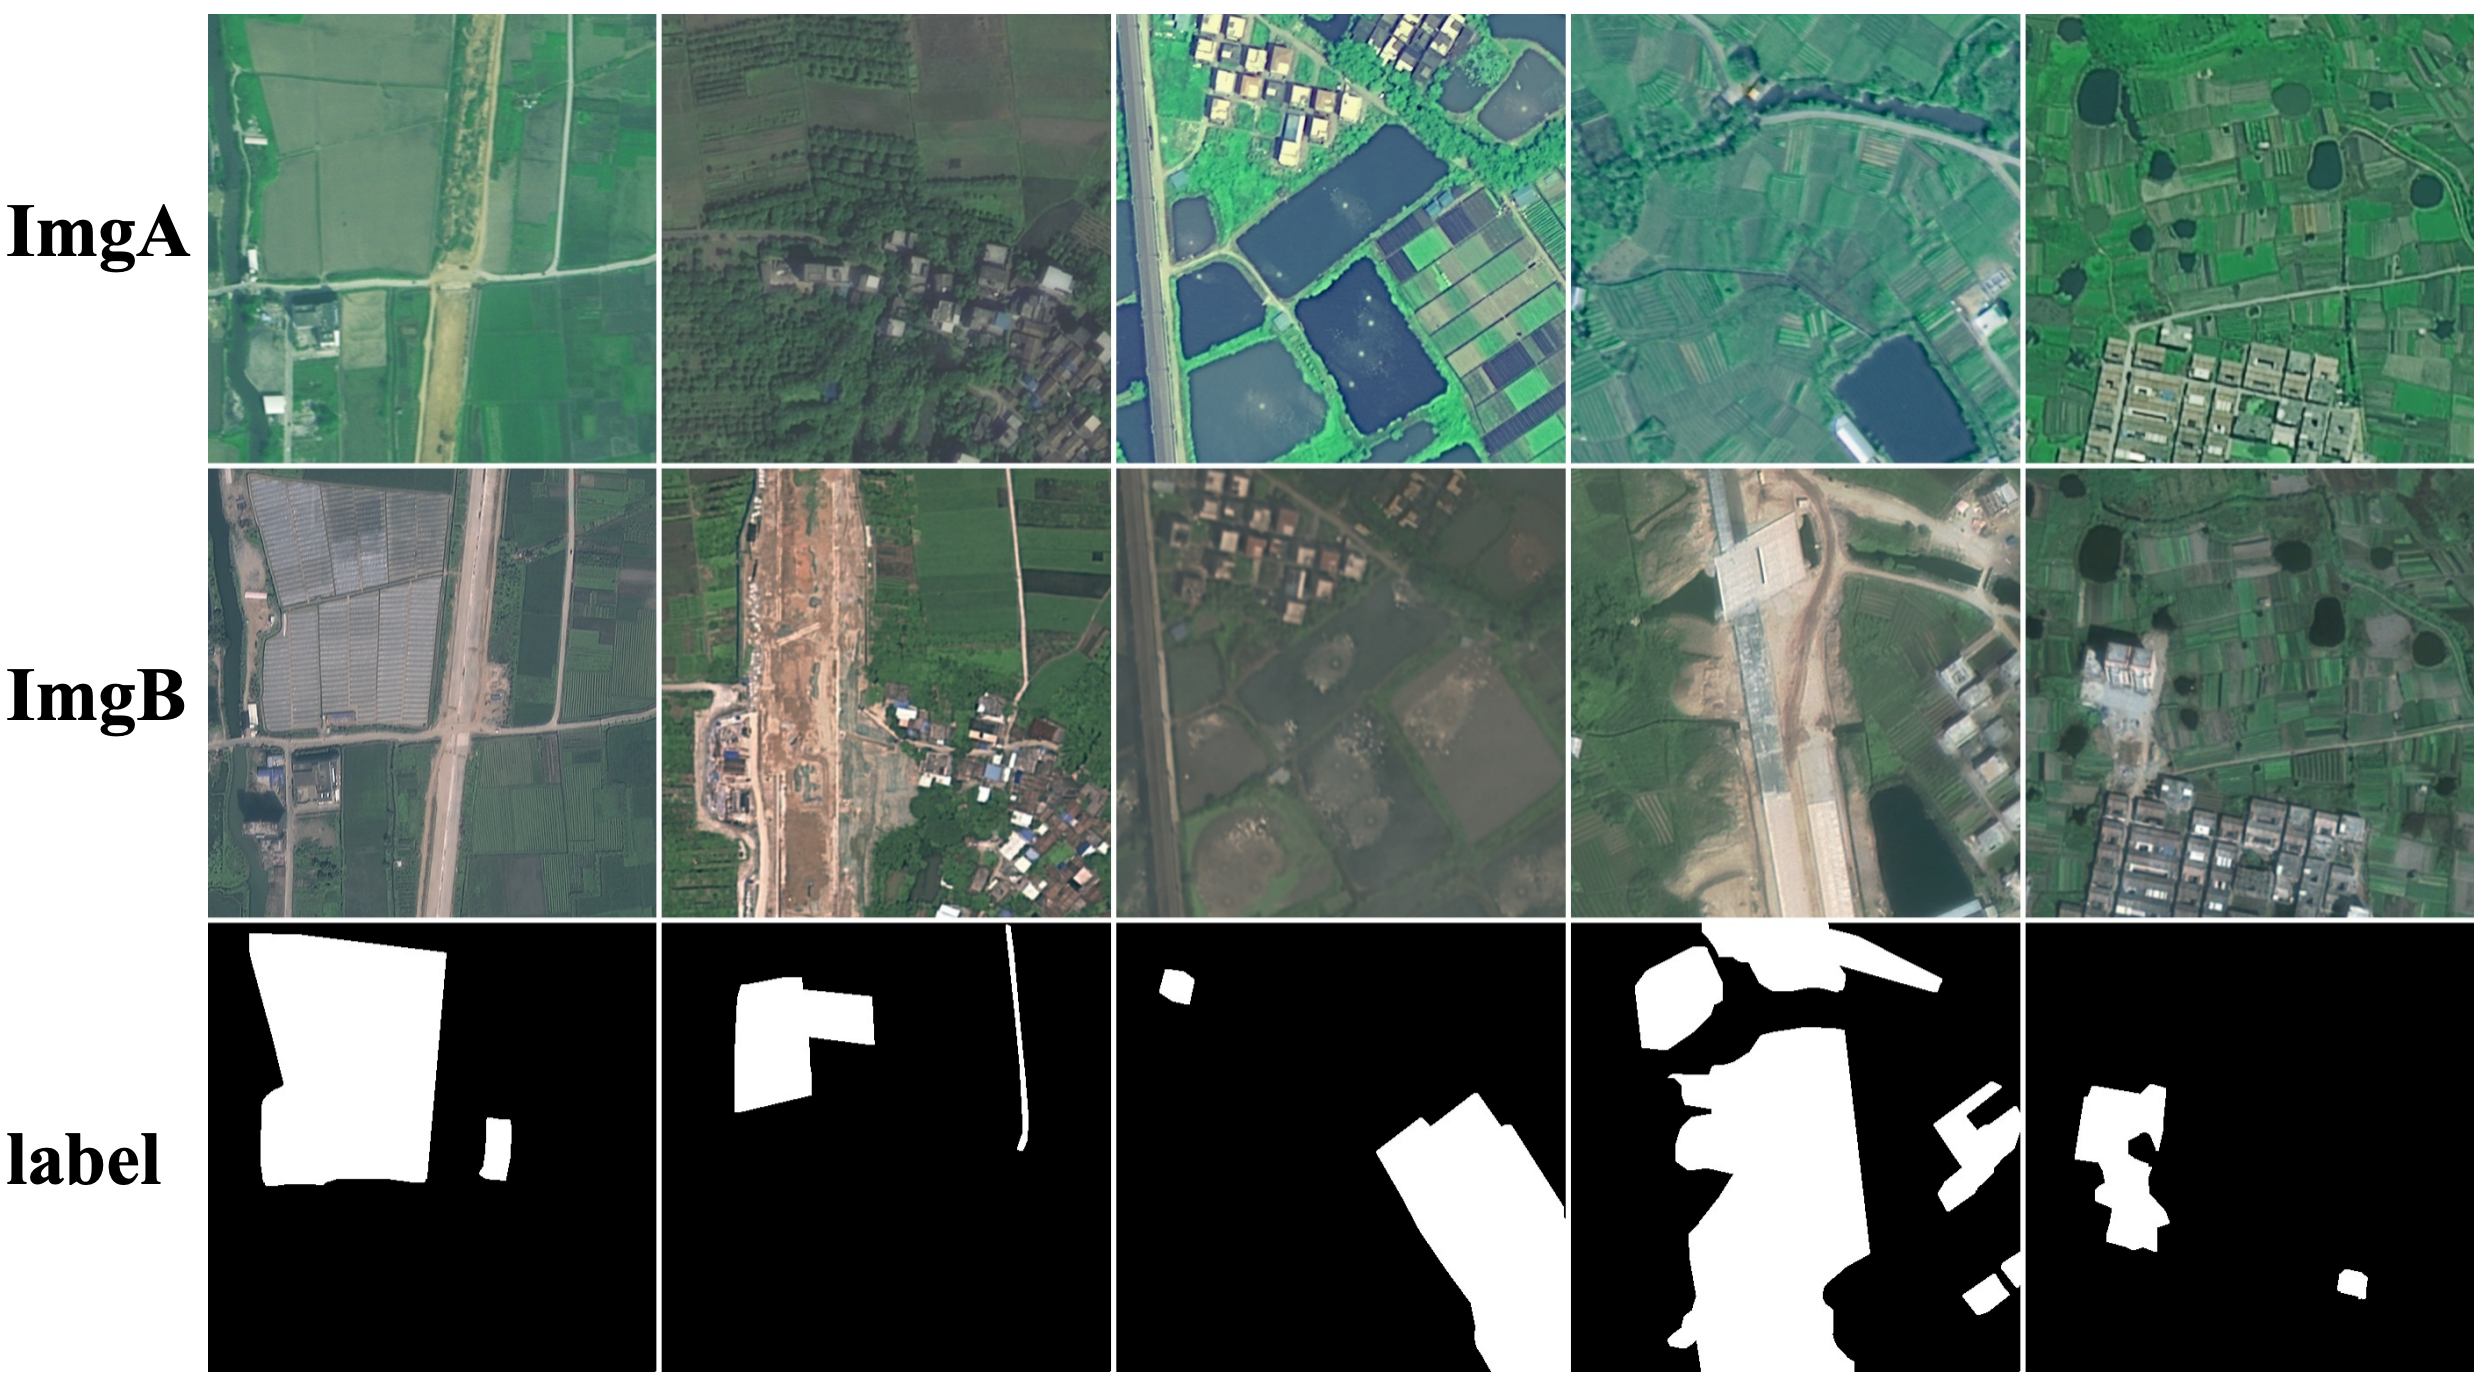
\includegraphics[width=0.75\textwidth]{paper_figures/变化检测任务与实验方法介绍/clcd.png}
  \caption{CLCD 数据集展示.}
  \label{fig:clcd}
\end{figure}

\subsubsection{PX-CLCD数据集}
Peixian耕地变化检测(PX-CLCD)数据集~\cite{miao_snunet3_2024}最初包含5170对具有1米空间分辨率、256×256像素的双时相图像。在数据集的构建过程中,按照6:2:2的比例将数据集划分为训练集、验证集和测试集。为了扩充数据集,研究人员通过应用随机翻转和旋转等数据增强技术,最终生成了PX-CLCD耕地变化检测数据集,分别代表2018年和2021年两年的耕地变化图像。如图~\ref{fig:pxclcd}所示,PX-CLCD数据集的变化类型主要包括耕地上新建温室、耕地上新修硬化道路、耕地上新建人工湖以及耕地上新建房屋等,这些变化类型在数据集中均得到了详细标注。

\begin{figure}[!htbp]
  \centering
  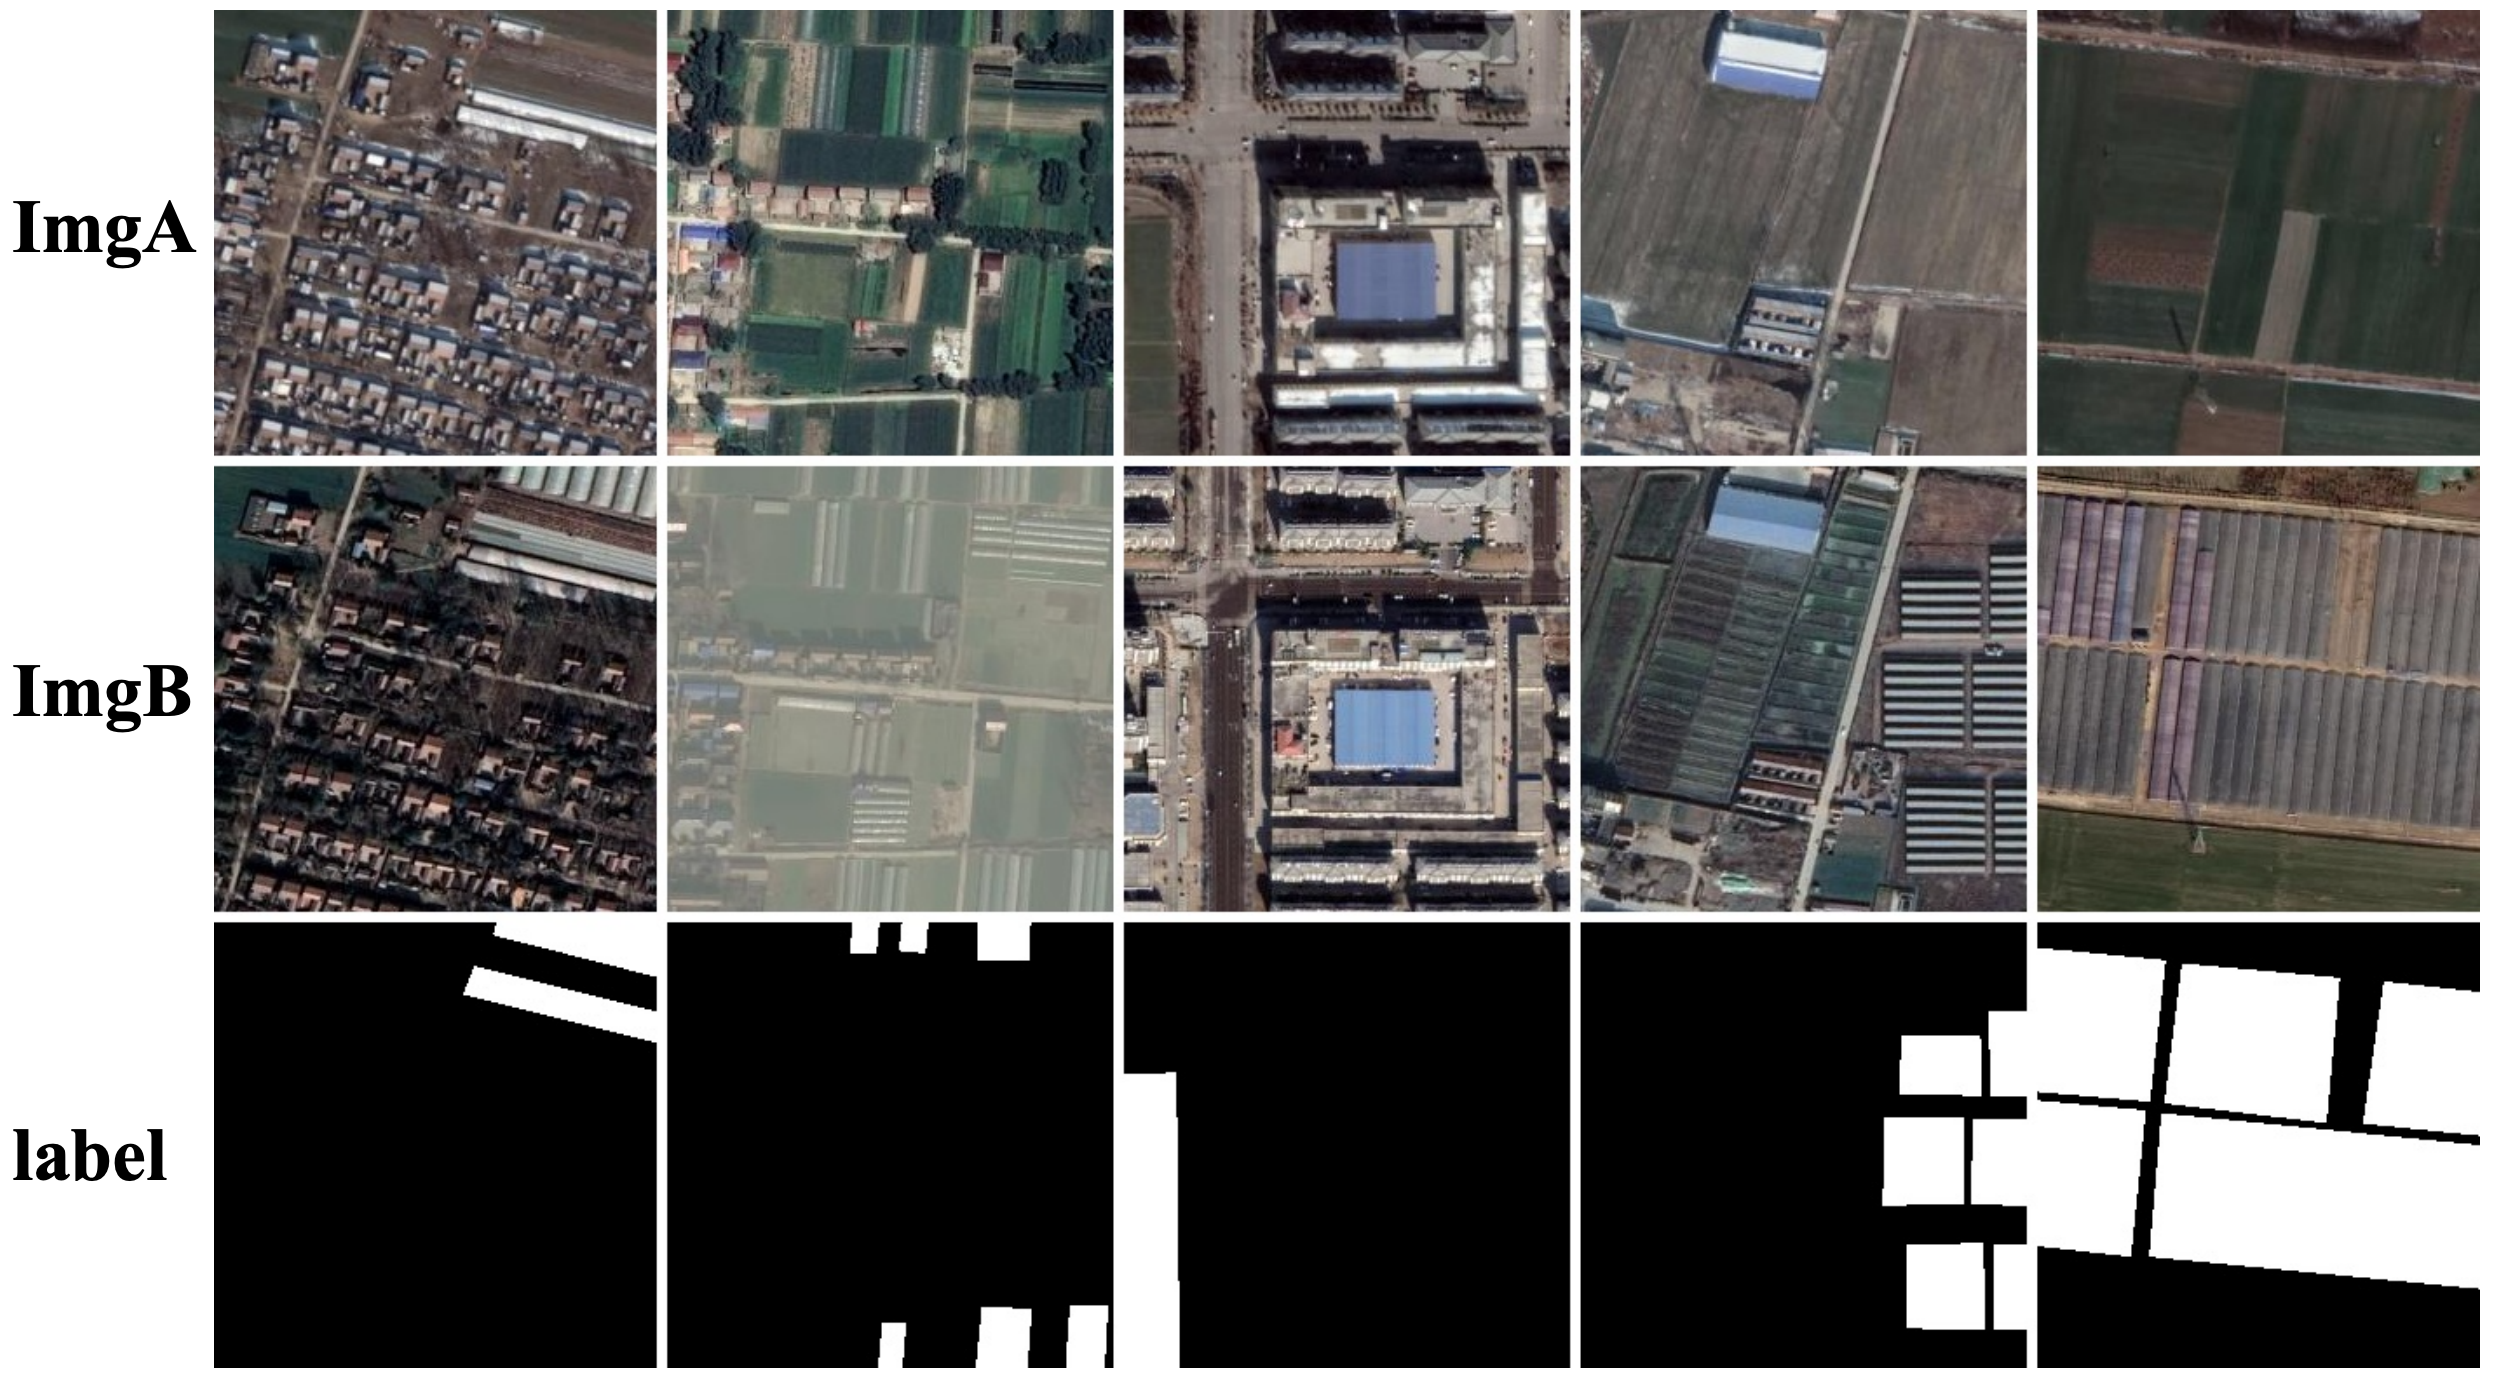
\includegraphics[width=0.75\textwidth]{paper_figures/变化检测任务与实验方法介绍/pxclcd.png}
  \caption{PX-CLCD 数据集展示.}
  \label{fig:pxclcd}
\end{figure}

\subsection{针对水体区域的变化检测数据集}
Water-CD 数据集~\cite{j_li_trsanet_2024}旨在促进水体变化检测,填补了变化检测任务在水体变化检测中的空白。如图~\ref{fig:watercd}所示,Water-CD 数据集包含来自中国长江流域的季节性湖泊,以及南亚朱姆纳河等地的各种季节性水体。Water-CD数据集卫星影像获取了空间分辨率为 10 m 的双时相遥感数据,包含红光(R)、绿光(G)和近红外(NIR)波段,影像均为 2016–2022 年间雨季和旱季拍摄的无云图像。Water-CD水体变化检测图像数据集包含 1149 对双时相影像,每对影像的尺寸为 512 × 512。

\begin{figure}[!htbp]
  \centering
  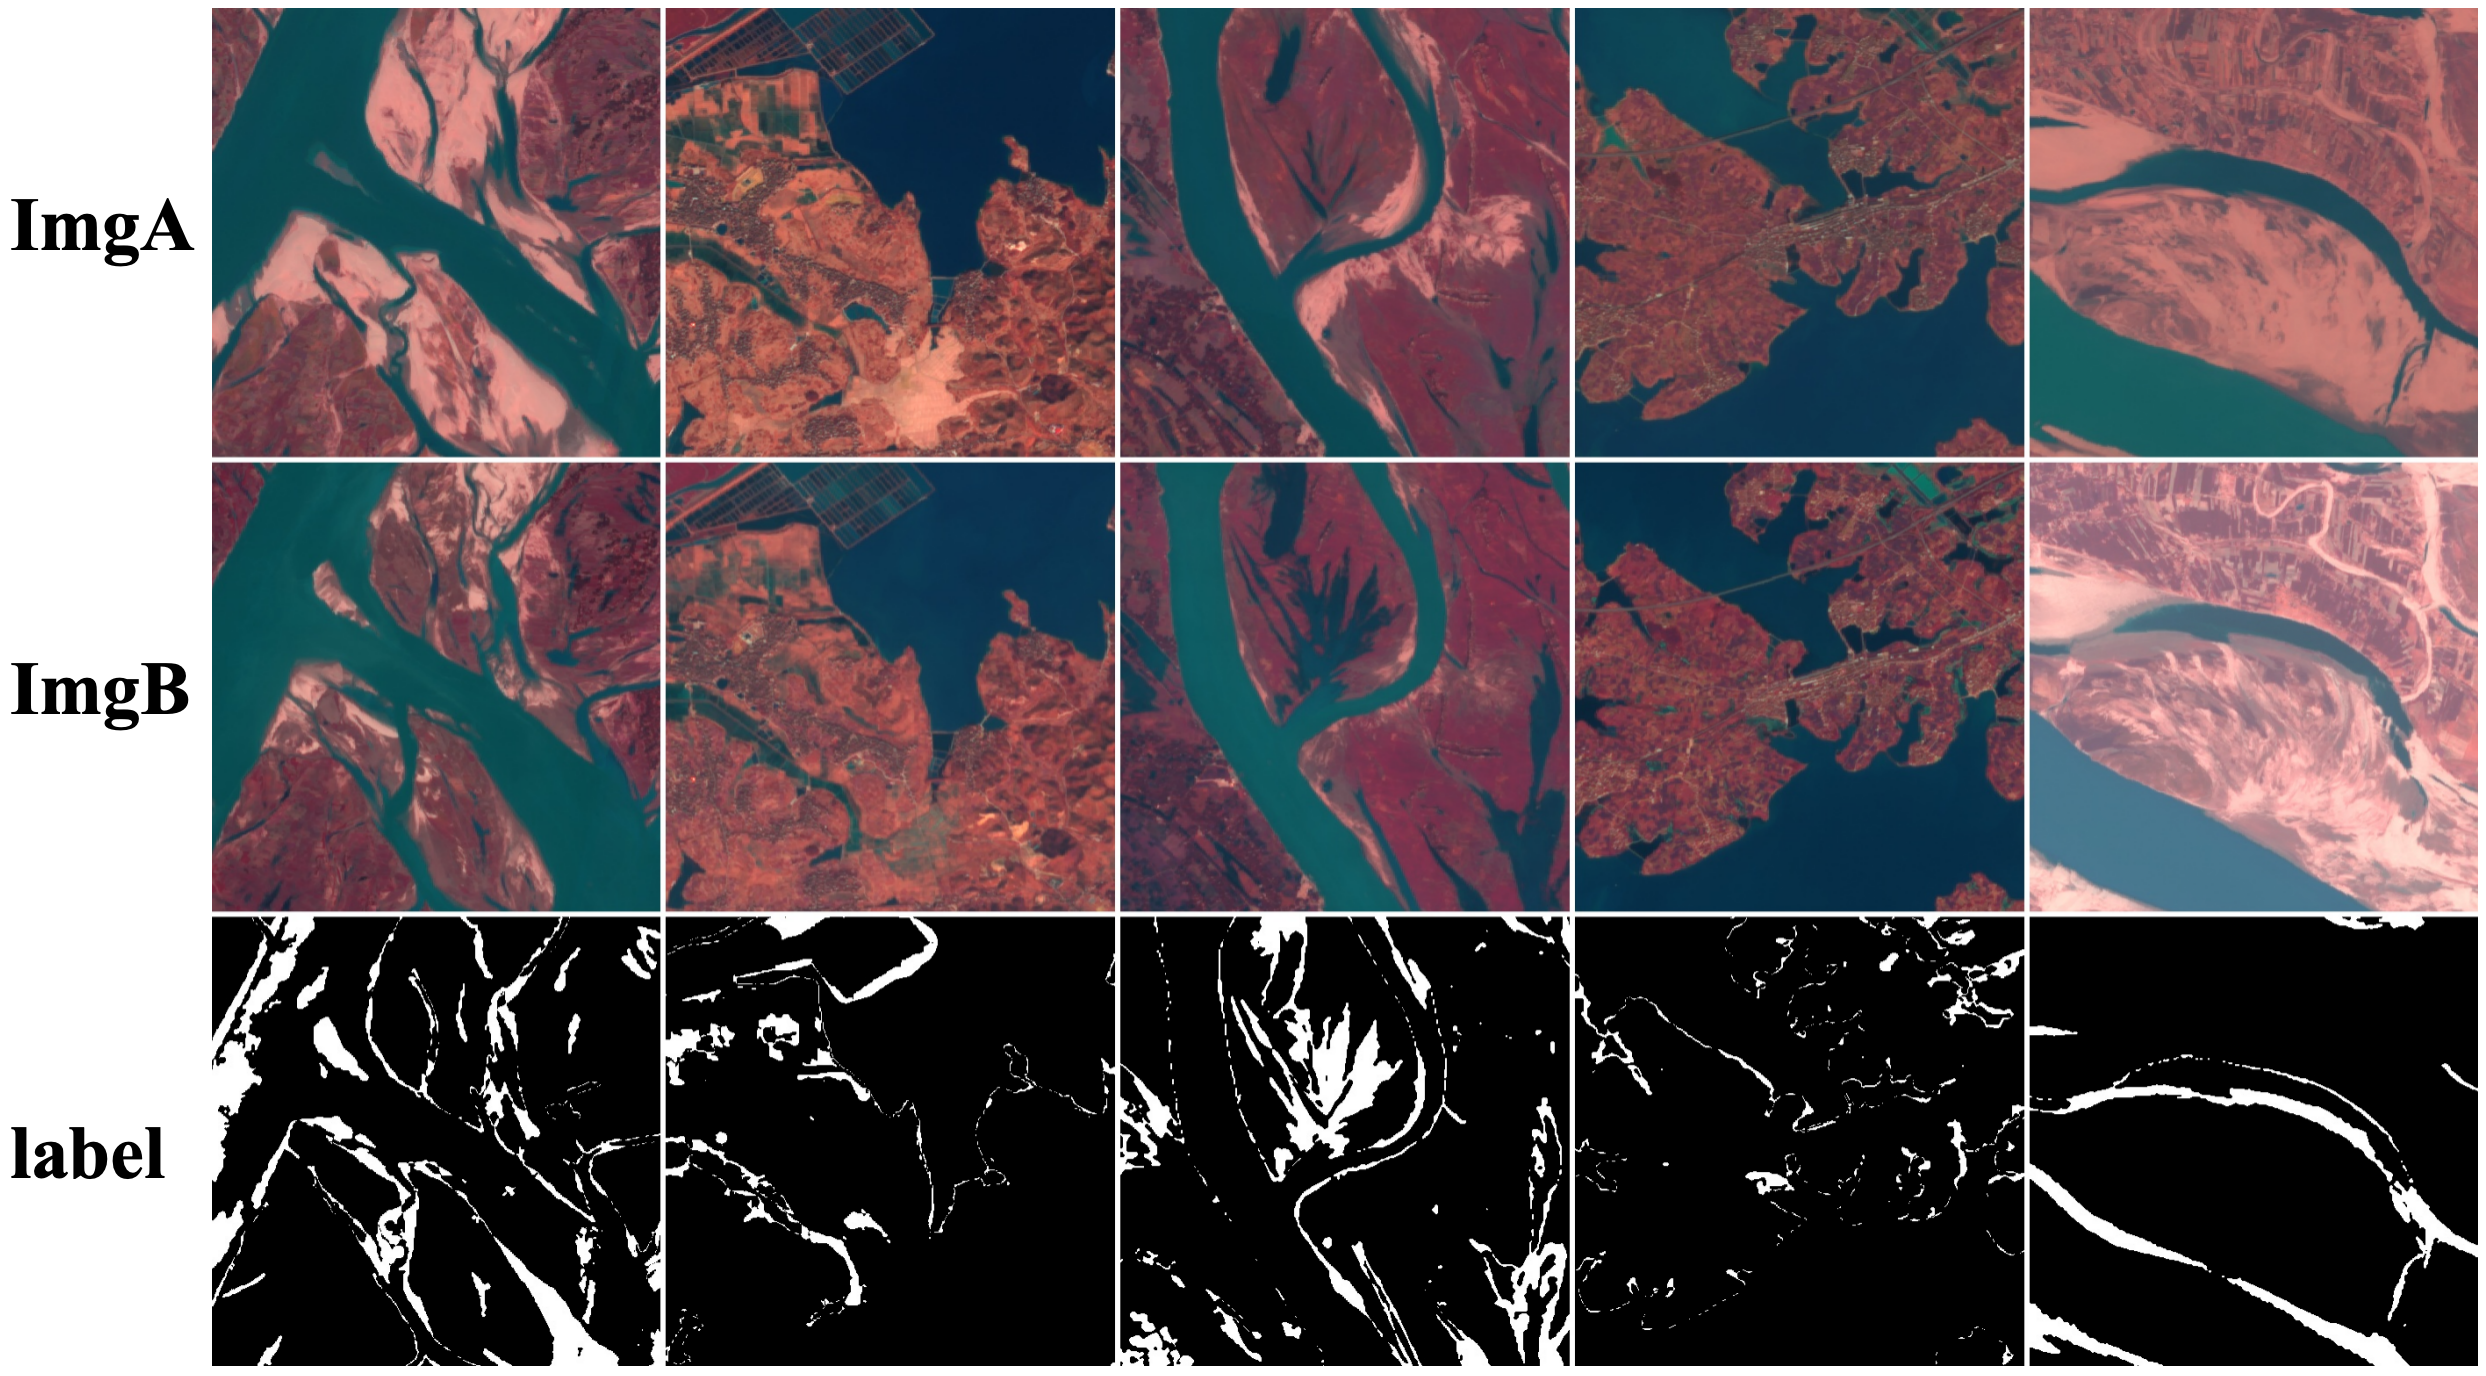
\includegraphics[width=0.75\textwidth]{paper_figures/变化检测任务与实验方法介绍/watercd.png}
  \caption{Water-CD 数据集展示.}
  \label{fig:watercd}
\end{figure}

\subsection{通用变化检测数据集}
\subsubsection{CDD数据集}
CDD变化检测数据集~\cite{Lebedev2018CHANGEDI}包含显示同一区域季节变化的卫星图像。该数据集通过收集来自Google Earth的数据创建,包括分辨率范围从0.03米到1米的图像。数据集中的图像被随机裁剪为256×256的大小。裁剪后,数据集被划分为训练集、验证集和测试集。训练集包含10000张图像,而验证集和测试集各包含3000张图像。该数据集旨在测试变化检测模型在同一区域随时间变化时识别变化的能力。如图~\ref{fig:cdd}所示,数据集包含多种变化类型,如城市发展、植被变化和水体变化,因此它是评估变化检测模型在不同场景下表现的有用工具。

\begin{figure}[!htbp]
  \centering
  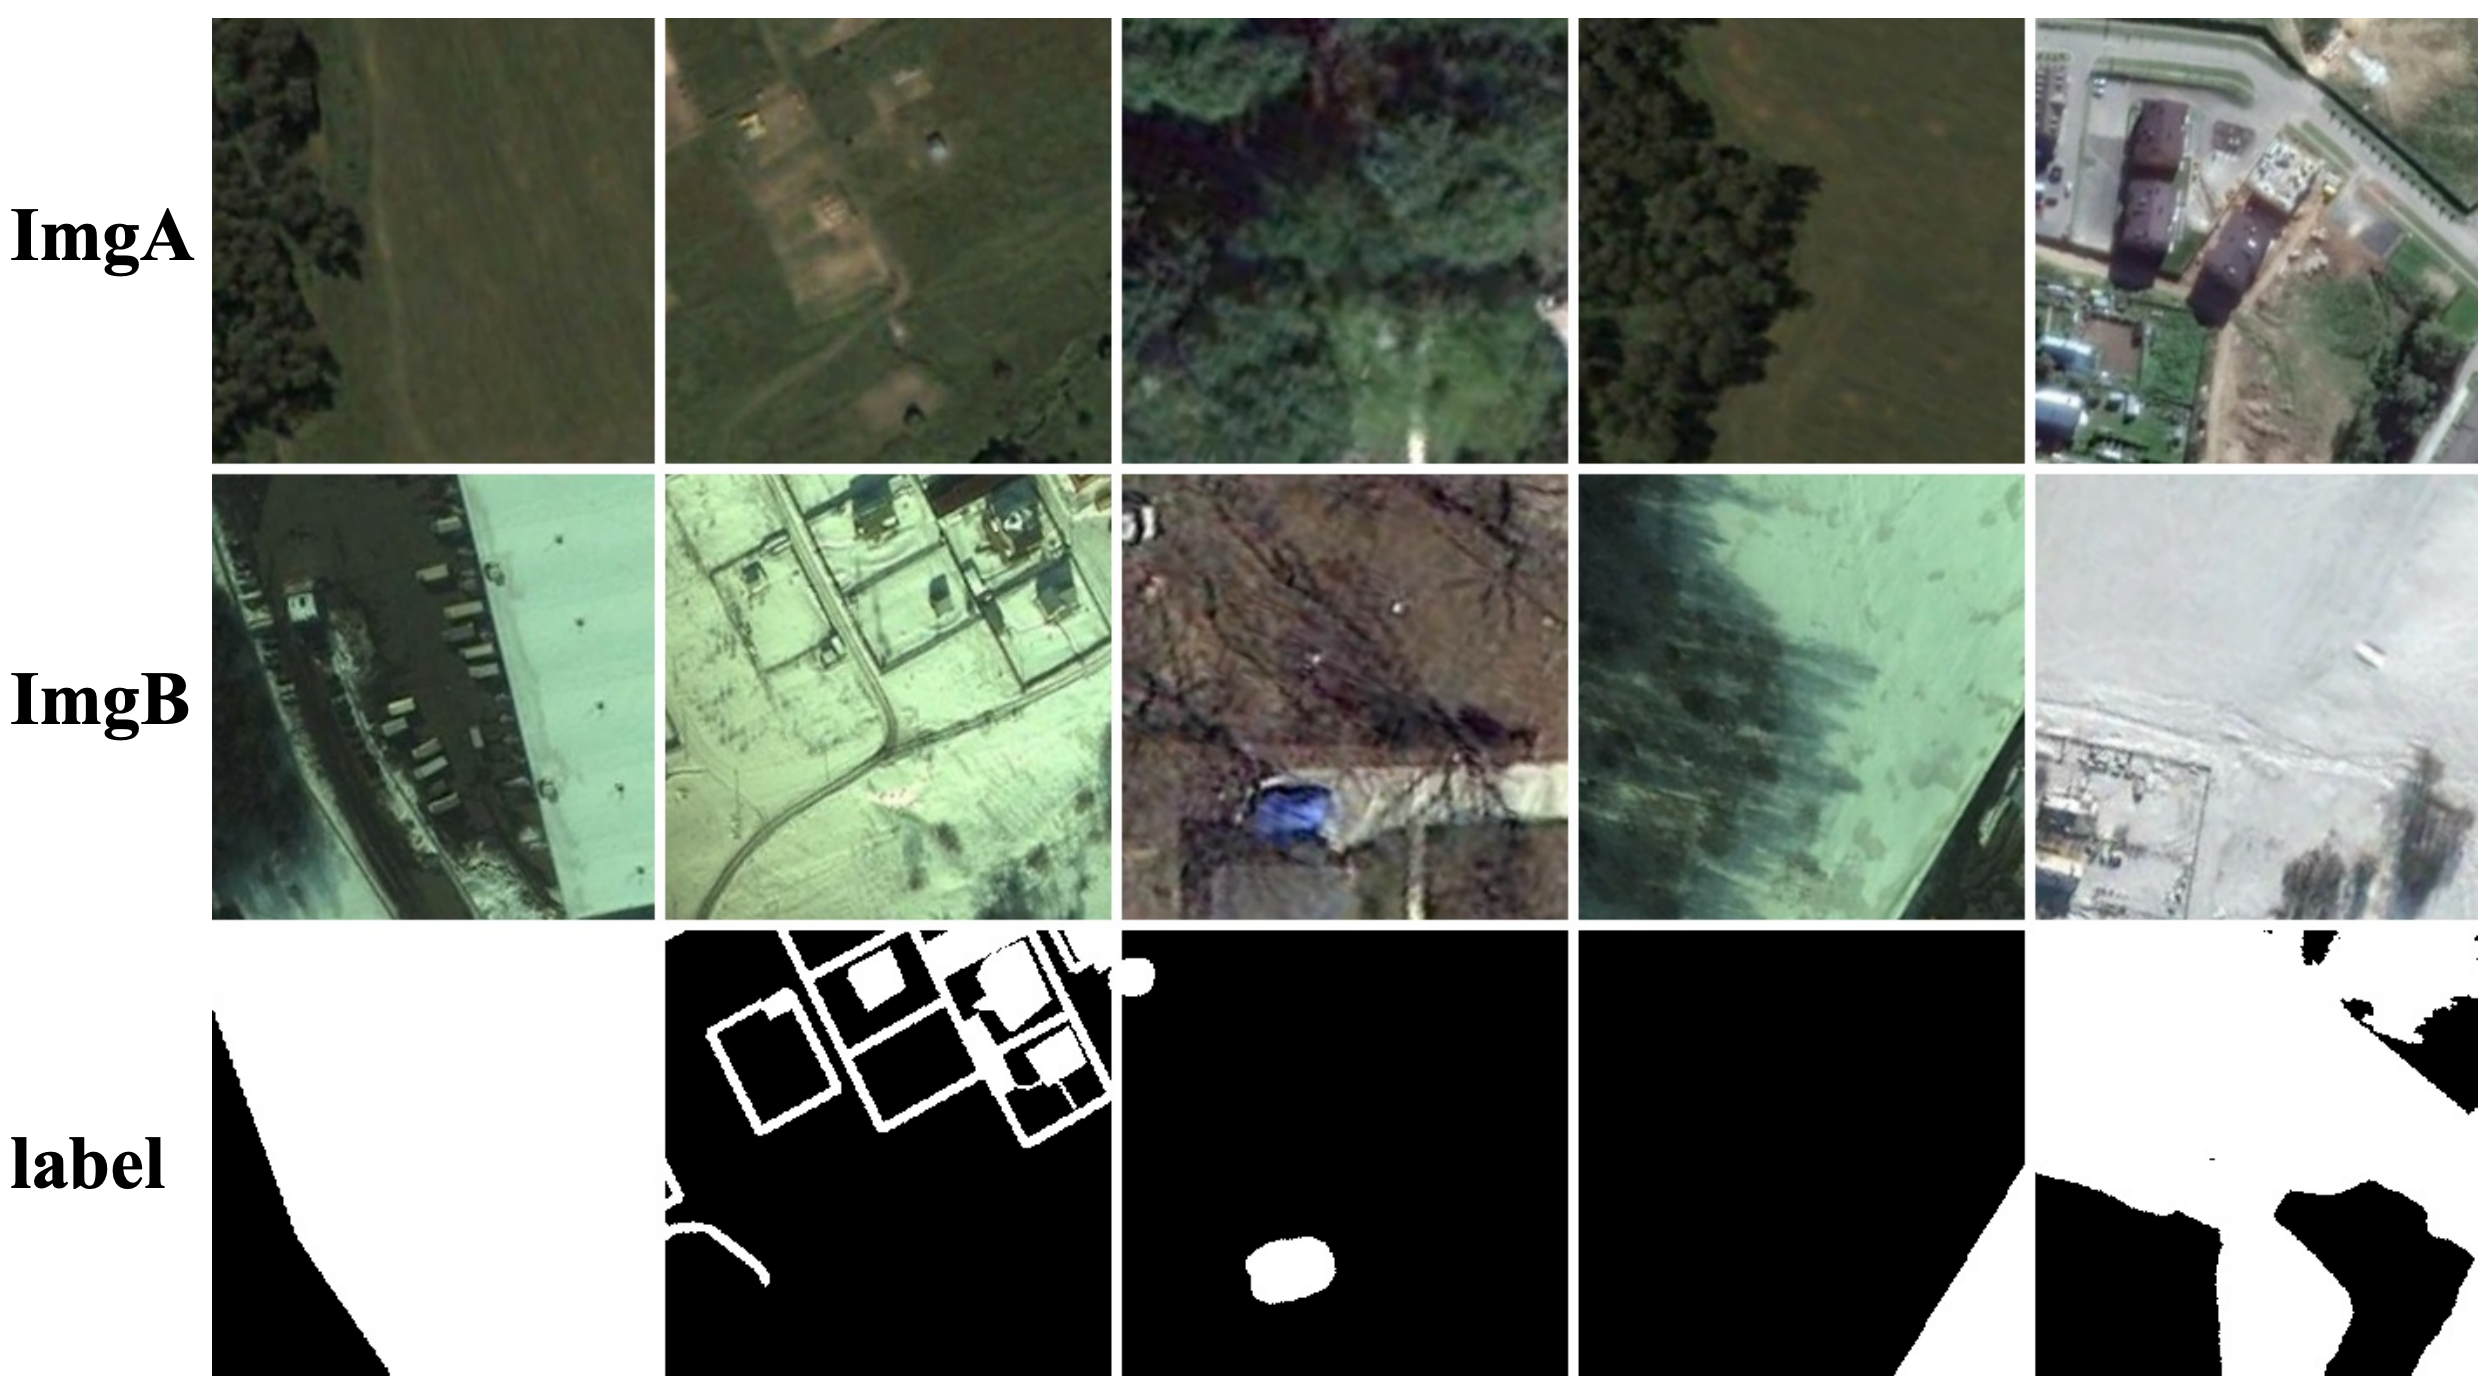
\includegraphics[width=0.75\textwidth]{paper_figures/变化检测任务与实验方法介绍/cdd.png}
  \caption{CDD 数据集展示.}
  \label{fig:cdd}
\end{figure}

\subsubsection{SYSU数据集}
SYSU-CD数据集~\cite{shi_deeply_2022}是一个包含20000对高分辨率航拍图像的集合,每张图像大小为256×256像素,图像采集自2007至2014年间的香港。该数据集包含多种变化类型,包括新建城市建筑、郊区扩展、建设前的地面准备、植被变化、道路扩展以及海上建筑等。如图~\ref{fig:sysu}所示,SYSU-CD数据集高度代表了城市变化,涵盖了大多数在城市环境中发生的变化类型。该数据集被划分为三部分:训练集、验证集和测试集,分别包含12000对、4000对和4000对图像。这种划分遵循了常用的实验程序。SYSU-CD数据集为评估和比较不同类型城市变化的变化检测算法性能提供了宝贵的资源。

\begin{figure}[!htbp]
  \centering
  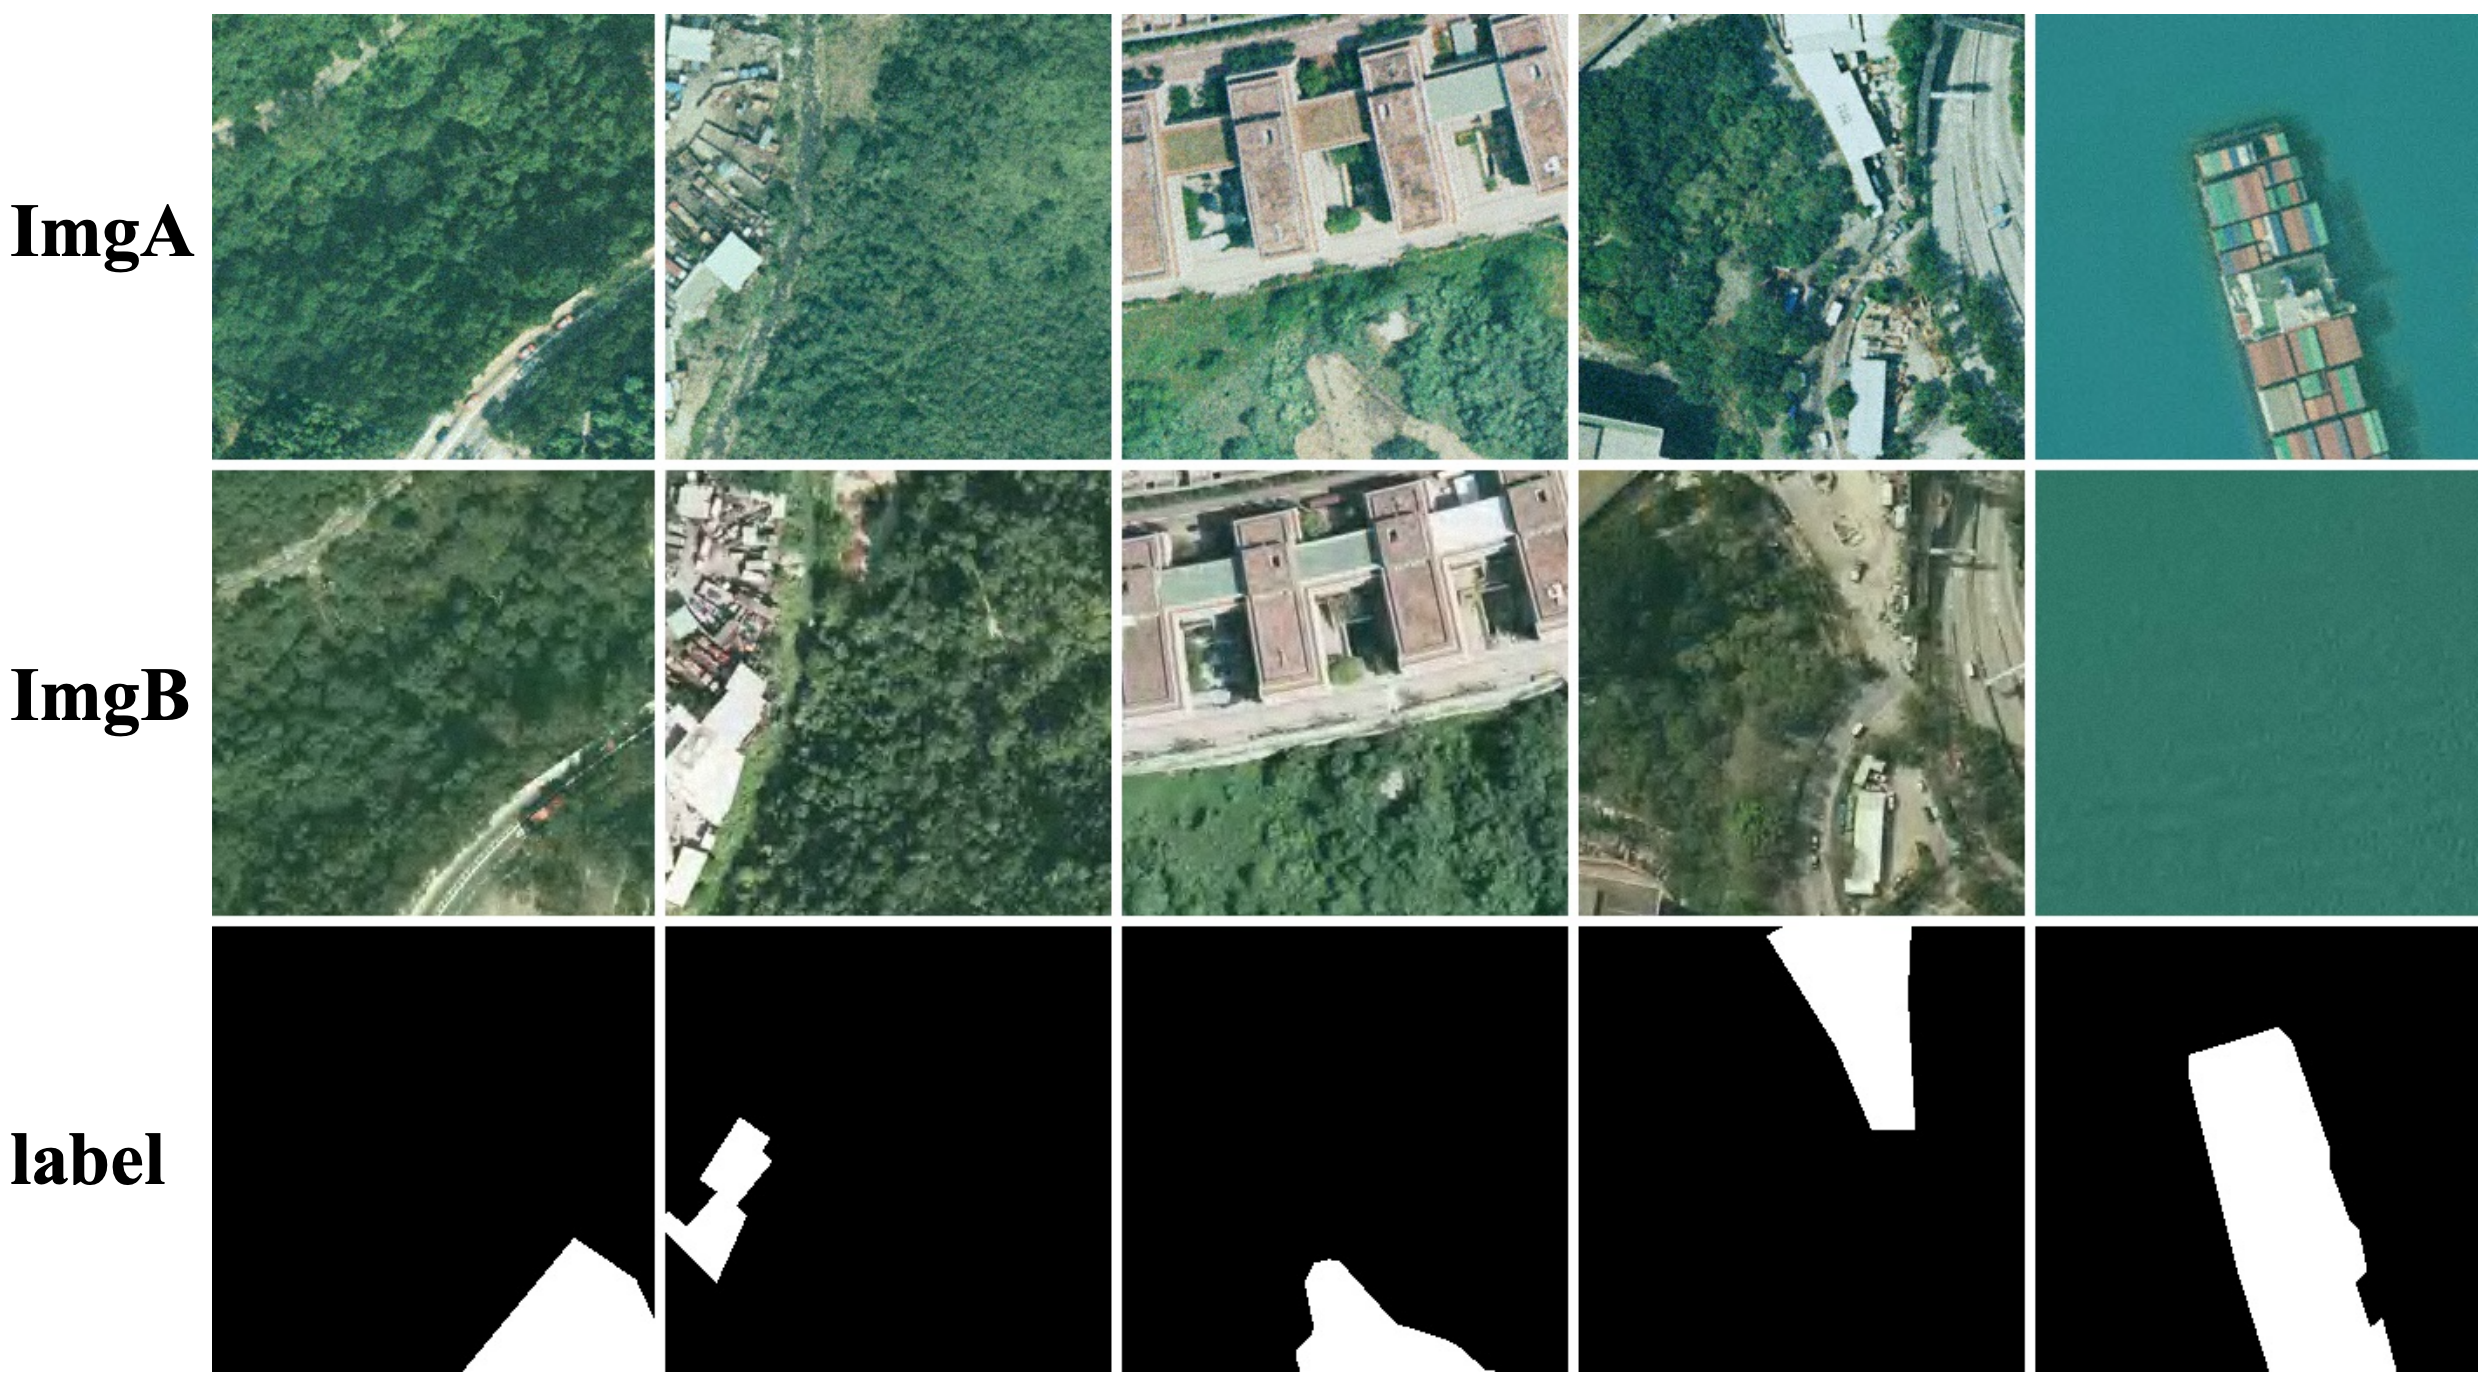
\includegraphics[width=0.75\textwidth]{paper_figures/变化检测任务与实验方法介绍/sysu.png}
  \caption{SYSU-CD 数据集展示.}
  \label{fig:sysu}
\end{figure}

\begin{figure}[!htbp]
  \centering
  \includegraphics[width=0.75\textwidth]{paper_figures/变化检测任务与实验方法介绍/msrscd.png}
  \caption{MSRSCD 数据集展示.}
  \label{fig:msrscd}
\end{figure}


\subsubsection{MSRSCD数据集}
MSRSCD数据集~\cite{Liu2025NetworkAD}在图像分辨率、变化类型、数据集大小和变化维度方面显著补充了现有的遥感影像变化检测数据集,进一步为变化检测任务提供了新的基准。该数据集包括2019年至2023年间在中国南方城市捕获的841对遥感图像,每张图像大小为1024×1024像素,空间分辨率为0.5米。数据集按照7:1:2的比例分为训练集、验证集和测试集。如图~\ref{fig:msrscd}所示,数据集中的主要变化类型包括新建筑、郊区扩张、植被变化和道路建设。

\begin{figure}[!htbp]
  \centering
  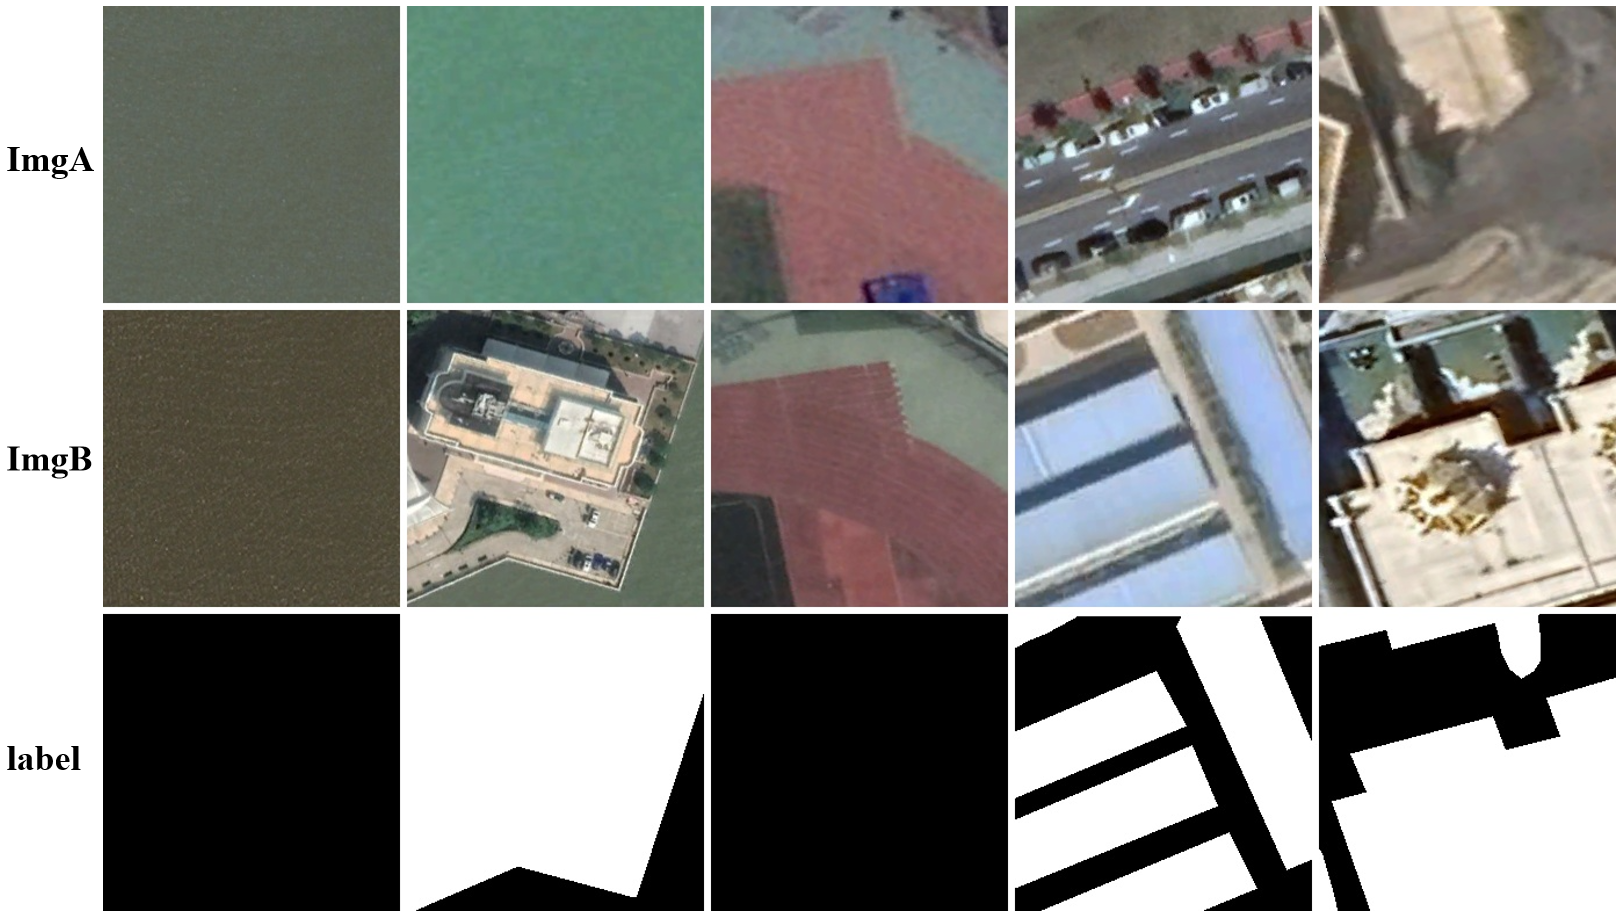
\includegraphics[width=0.75\textwidth]{paper_figures/变化检测任务与实验方法介绍/mlcd.png}
  \caption{MLCD 数据集展示.}
  \label{fig:mlcd}
\end{figure}

\subsubsection{MLCD数据集}
MLCD数据集~\cite{Huang2025SAMBasedEF}(Macao Land Change Detection)聚焦于澳门地区2008至2023年间的土地填海与植被动态变化,基于Google Earth Engine影像构建。如图~\ref{fig:mlcd}所示,该数据集包含10,000对已标注的$256\times256$遥感影像,空间分辨率为0.5–2米,为海岸地貌与土地利用演变研究提供了新的基准。


\begin{table}[!htbp]
\centering
\caption{本文所选用的遥感影像变化检测数据集概览}
\label{tab:change_detection_datasets_review}
\setlength{\tabcolsep}{4pt} % 列间距紧凑一些
\renewcommand{\arraystretch}{1.15}
\small
\begin{tabularx}{\textwidth}{@{} l c c c X X c @{}}
\toprule
\textbf{数据集} & \textbf{切片尺寸} & \textbf{数据总量} & \textbf{影像分辨率} & \textbf{影像地理位置} & \textbf{卫星} & \textbf{应用对象} \\
\midrule
LEVIR-CD~\cite{chen_spatial-temporal_2020}   & 1024$\times$1024 & 637    & 0.5 m        & American cities                                   & Google Earth                     & 建筑物 \\
LEVIR-CD+~\cite{chen_spatial-temporal_2020}  & 1024$\times$1024 & 985    & 0.5 m        & American cities                                   & Google Earth                     & 建筑物 \\
WHUCD~\cite{Ji2019FullyCN}     & 256$\times$256   & 7620   & 0.2 m        & Christchurch, New Zealand                          & --                                & 建筑物 \\
S2Looking~\cite{Shen2021S2LookingAS}  & 1024$\times$1024 & 5000   & 0.5--0.8 m   & --                                                & GaoFen / SuperView / BeiJing-2   & 建筑物 \\
MSRSCD~\cite{Liu2025NetworkAD}     & 1024$\times$1024 & 841    & 0.5 m        & Southern Chinese cities                           & --                                & 全场景 \\
SYSU-CD~\cite{shi_deeply_2022}    & 256$\times$256   & 20{,}000 & 0.5 m       & Hong Kong                                         & --                                & 全场景 \\
CDD~\cite{Lebedev2018CHANGEDI}        & 256$\times$256   & 16{,}000 & 0.03--0.1 m & --                                                & Google Earth                     & 全场景 \\
CLCD~\cite{Liu2022ACN}       & 512$\times$512   & 600    & 0.5--2 m     & Guangdong                                         & Gaofen-2                         & 耕地 \\
PX-CLCD~\cite{miao_snunet3_2024}    & 256$\times$256   & 5170   & 0.5--1 m     & Jiangsu                                           & Gaofen-2                         & 耕地 \\
Water-CD~\cite{j_li_trsanet_2024}   & 512$\times$512   & 1149   & 10 m         & Yangtze River; George Lake; Jamuna River          & Sentinel-2                       & 水体 \\
MLCD~\cite{Huang2025SAMBasedEF}       & 256$\times$256   & 10{,}000 & 0.5--2 m    & Macao                                             & Google Earth                     & 全场景 \\
\bottomrule
\end{tabularx}
\end{table}


如表~\ref{tab:change_detection_datasets_review}所示,总结了本文选取的当前主流变化检测数据集及其基本信息。这些数据集在多个维度上展现了高度的多样性,为全面评估算法性能提供了坚实基础。在应用对象上,既包括专注于建筑物变化的LEVIR-CD、WHU-CD与S2Looking数据集,也有面向耕地(CLCD、PX-CLCD)与水体(Water-CD)等特定自然资源监测的数据集,更有涵盖多种变化类型的全场景数据集(MSRSCD、SYSU-CD、CDD、MLCD)。在技术参数上,空间分辨率覆盖了从10米(Water-CD)的中等分辨率到亚米级乃至厘米级(如WHU-CD的0.2米和CDD的0.03米)的高分辨率影像;数据总量也从数百对样本的CLCD到两万对样本的SYSU-CD不等,充分考验了算法在不同数据规模下的性能。此外,这些数据集在地理范围与传感器类型上也极具代表性,地理上横跨了北美城市、新西兰、中国香港及内地多个省份,数据来源则涵盖了谷歌地球(Google Earth)、高分系列(Gaofen-2)、哨兵系列(Sentinel-2)等多种平台。这种多维度、多层次的多样性确保了本文的实验评估具有广泛的代表性,能够全面检验本文所提模型在不同场景、不同尺度和不同数据条件下的适应性与泛化能力。

\section{变化检测实验方法介绍}
\subsection{变化检测训练策略}
在遥感影像变化检测任务中,深度学习方法已经成为主流。为了使模型能够在不同类型和场景的变化检测任务中表现出色,合理的训练策略与数据增强方法至关重要。良好的训练策略不仅能够加速模型的收敛过程,还能提升模型的泛化能力;而数据增强则通过合成多样化的训练样本,提高模型在复杂场景下的鲁棒性,有效缓解过拟合问题。以下从训练集构建、模型设计、数据增强、损失函数以及优化策略等方面总结常用做法。

变化检测的训练策略通常包括训练集的构建、损失函数的设计以及优化策略的选择。为确保模型能够准确检测变化区域并实现有效分类,训练过程中的设计需要重点关注以下几个方面:
\begin{itemize}
 \item \textbf{训练集的构建}:在构建训练集时,应保证双时相影像来自同一地区,具有配准的地理坐标。此外,为了提高数据的多样性,可以通过裁剪大尺寸影像得到小块样本,从而提升模型的学习效率。
 
 \item \textbf{变化检测模型设计}:模型的设计通常采用孪生结构(Siamese Network)或编码-解码结构,以便有效提取和对比双时相影像特征。近年来,加入注意力机制、多尺度特征融合与特征交互模块的设计能够进一步提升模型对细粒度变化的感知能力。
 
 \item \textbf{数据增强策略}:常见的数据增强方法包括旋转、翻转、镜像以及色彩抖动等。这些操作可以增加样本多样性,使模型更好地适应不同光照、季节和传感器条件下的影像变化。
 
 \item \textbf{损失函数的设计}:损失函数通常采用交叉熵损失、Dice Loss 或两者的组合,以兼顾像素级分类精度与变化区域的整体一致性。在一些方法中,还会引入边界约束损失或对比损失,以增强模型对边界细节与类别差异的刻画能力。
 
 \item \textbf{优化策略的选择}:优化器一般选用Adam或AdamW,并结合余弦退火或多步学习率下降策略,以实现更稳定的收敛过程。同时,可采用早停(Early Stopping)机制,避免模型在后期出现过拟合。
\end{itemize}


\subsection{变化检测数据增强}
数据增强是深度学习中常用的技术,旨在通过人为生成新的训练样本,扩大训练集的多样性,从而提高模型的鲁棒性和泛化能力。在遥感影像变化检测任务中,数据增强的主要目标是模拟各种可能的变化场景,帮助模型在面对不同的环境条件时仍然能保持良好的性能。常见的变化检测数据增强方法包括:

\textbf{几何变换}:几何变换通过对图像进行旋转、缩放、翻转和裁剪等操作,模拟不同视角和尺度下的变化。通过这种方式,模型能够学习到变化区域在不同视角和不同分辨率下的表现,从而提升模型对这些变化的识别能力。尤其是在多时相影像变化检测任务中,图像的旋转和裁剪能够有效地模拟不同时间点拍摄的影像之间的几何差异。

\textbf{光照变化}:由于遥感影像的拍摄时间、季节以及天气条件的不同,光照变化对图像的影响是不可忽视的。通过对图像的亮度、对比度和饱和度进行调整,数据增强方法可以模拟不同光照条件下的影像变化。这有助于模型学习到变化区域在不同光照下的表现,增加其在不同环境条件下的鲁棒性。

\textbf{噪声添加}:遥感影像中经常存在各种噪声,包括盐噪声、椒噪声和高斯噪声等。通过在图像中加入不同类型的噪声,数据增强可以模拟传感器噪声和环境干扰。这有助于提高模型在实际应用中对噪声的处理能力,使其在高噪声环境下仍然能够准确检测到变化区域。

\textbf{图像变换和混合}:图像变换技术,如图像融合、样式转换(style transfer)和伪标签生成等方法,能够进一步丰富训练样本的多样性。例如,利用生成对抗网络(GAN)生成样式相似但内容不同的影像,可以为模型提供更多样化的变化场景。另外,图像混合方法(如Mixup)也可以通过将两幅图像的像素值加权混合,合成出新的训练样本,进一步提高模型对变化区域的感知能力。

\textbf{随机裁剪与填充}:随机裁剪可以帮助模型聚焦于局部区域的变化,这对于提高模型在变化细节处理上的能力至关重要。此外,在进行裁剪时,通常还会在裁剪后的图像中进行填充操作,确保输入图像的尺寸一致,这有助于网络保持输入图像的尺寸一致性。



\begin{sidewaystable}[htbp]
\centering
\scriptsize
\caption{不同研究侧重的变化检测模型汇总}
\label{tab:cd_models_summary}
\begin{tabularx}{\textheight}{@{}l X@{}} % 注意这里要用 \textheight 替代 \textwidth
\toprule
\textbf{研究侧重} & \textbf{模型汇总} \\
\midrule
结合CNN & CDNet~\cite{Alcantarilla2016StreetviewCD}、FC-Siam-Di~\cite{Daudt2018FullyCS}、FresUNet~\cite{Daudt2018MultitaskLF}、L-UNet~\cite{Papadomanolaki2021ADM}、DTCDSCN~\cite{Liu2019BuildingCD}、P2V~\cite{lin_transition_2023}、JFSDNet~\cite{Zhou2022JointFD}、LGPNet~\cite{Liu2022BuildingCD}、AFCF3D-Net~\cite{Ye2023AdjacentLevelFC}、STFF-GA~\cite{h_wei_spatio-temporal_2024}、AMFNet~\cite{zhan_amfnet_2024}、TRSANet~\cite{j_li_trsanet_2024}、HANet~\cite{Han2024HANetAH}、AFCF3DNet~\cite{ye_adjacent-level_2023}、AGFormer~\cite{Chen2025AGFormerAA}、SGSLN~\cite{zhao_exchanging_2023}、FCCDN~\cite{Chen2021FCCDNFC}、AANet~\cite{Hang2024AANetAA}、EfficientCD~\cite{dong_efficientcd_2024}、SSCD~\cite{Wang2024SummatorSubtractorNM}、MSCANet~\cite{m_liu_cnn-transformer_2022}\\
\midrule
结合注意力机制 & STANet~\cite{chen_spatial-temporal_2020}、HMCNet~\cite{Wang2022HMCNetHE}、DMATNet~\cite{Song2022RemoteSI}、DSAMNet~\cite{shi_deeply_2022}、IRA-MRSNet~\cite{Ling2022IRAMRSNetAN}、ISDANet~\cite{h_ren_interactive_2025}、HATNet~\cite{Xu2024HybridAT}、CDNeXt~\cite{wei_robust_2024}、DMINet~\cite{feng_change_2023}、BASNet~\cite{z_wang_bitemporal_2024}、AMTNet~\cite{Liu2023AnAM}、ACABFNet~\cite{Song2023AxialCA}、ACAHNet~\cite{Zhang2023AsymmetricCH}\\
\midrule
结合Transformer & BIT~\cite{chen_remote_2022}、MFATNet~\cite{Mao2022MFATNetMF}、ChangeFormer~\cite{bandara2022transformer}、HMCNet~\cite{Wang2022HMCNetHE}、TransUNetCD~\cite{Li2022TransUNetCDAH}、STransUNet~\cite{Yuan2022STransUNetAS}、SwinSUNet~\cite{zhang_swinsunet_2022}、RCDT~\cite{Lu2022RCDTRR}、DgFA~\cite{f_zhou_dual-granularity_2025}、FTransDF-Net~\cite{li_dual_2025}、ScratchFormer~\cite{Noman2023RemoteSC}、Conv-former~\cite{Yang2025ConvFormerCDHC}、EATDer~\cite{Ma2024EATDerEA}\\
\midrule
结合Mamba & CDMamba~\cite{zhang_cdmamba_2025}、RSM-CD~\cite{zhao_rs-mamba_2024}、CWmamba~\cite{Liu2025CWmambaLC}、CD-STMamba~\cite{Liu2025CDSTMambaTR}、HFIFNet~\cite{Han2025HFIFNetHF}、LCCDMamba~\cite{Huang2025LCCDMambaVS}、Hybrid-MambaCD~\cite{Feng2025HybridMambaCDHM}、ConMamba~\cite{Dong2024ConMambaCA}、FEMCD~\cite{Xing2025FrequencyEnhancedMF}、IMDCD~\cite{Liu2024IterativeMD}、MSA~\cite{Huang2025MSAMS}\\
\midrule
AI 基础模型 & SGANet~\cite{j_chen_sganet_2025}、SAM-Mamba~\cite{Li2025SAMMambaATC}、DepthCD~\cite{Zhou2025DepthCDDP}、EFI-SAM~\cite{Huang2025SAMBasedEF}、SAM-CD2~\cite{Sun2024SegmentAM}、DED-SAM~\cite{Qiu2025DEDSAMAdaptingSA}\\
\midrule
双时相特征融合 & SNUNet~\cite{Fang2021SNUNetCDAD}、DSIFN~\cite{Zhang2020ADS}、ICIF-Net~\cite{Feng2022ICIFNetIC}、DPCCNet~\cite{Papadomanolaki2021ADM}、DARNet~\cite{li_densely_2022}、ISNet~\cite{Cheng2022ISNetTI}、MFCF-Net~\cite{b_huang_remote-sensing_2024}、CMCD~\cite{li_cmcd_2025}、MIFNet~\cite{w_xie_mifnet_2025}、GASNet~\cite{zhang_global-aware_2023}、FHD~\cite{pei_feature_2022}、D-TNet~\cite{wan_d-tnet_2022-3}、SSANet~\cite{Jiang2022JointVL}、SFFCE-CD~\cite{y_xing_sffce-cd_2025}、FTA-Net~\cite{t_zhu_fta-net_2025}、HASNet~\cite{c_tao_hasnet_2025}、DDAM-Net~\cite{feng_ddam-net_2024}、SNUNet3+~\cite{miao_snunet3_2024}、CGNet~\cite{han_change_2023}、ELGCNet~\cite{m_noman_elgc-net_2024}、DEDANet~\cite{Li2025DifferenceEA}、DMFANet~\cite{Zhan2025DifferenceAwareMF}、SAFDNet~\cite{Fu2025BeyondCD}、AEGL-Net~\cite{Ying2025AEGLNetAM}、MSNet~\cite{Liu2025NetworkAD}、DFFNet~\cite{Liu2025FullScaleCD}、DSCRNet ~\cite{Zhang2025ADS}、B2CNet~\cite{Zhang2024B2CNetAP}、Changer~\cite{Fang2022ChangerFI}、MIN-Net~\cite{Zhou2024MultistageIN}、CACG-Net~\cite{Liu2024CandidateAwareAC}、PCAANet~\cite{Xu2023ProgressiveCA}、HCGMNet~\cite{Han2023HCGMNetAH}、STRobustNet~\cite{Zhang2025STRobustNetEC}\\
\midrule
新型架构 & STDF-CD~\cite{y_zhou_stdf_2025}、UA-BCD~\cite{li_overcoming_2025}、RSBuilding~\cite{wang_rsbuilding_2024}、MLDFNet~\cite{d_sidekejiang_mldfnet_2025}、DSFI-CD~\cite{x_li_dsfi-cd_2025}\\
\bottomrule
\end{tabularx}
\end{sidewaystable}

\subsection{变化检测性能评估方法}
为了验证本文提出的方法的有效性,本文与多种先进的变化检测方法进行了详细的对比。通过与先进变化检测模型在相同数据集上的性能比较,能够全面评估所提出方法的优势和创新点。对于每个数据集,计算了多个常用的评估指标,如交并比(IoU)、F1、精度(OA)、召回率(Rec)、精确率(Prec)。这些指标能够综合反映算法在不同类型变化区域上的检测能力和准确性。由于本文所针对的是通用变化检测模型,即分辨样本中发生变化的区域。通常这种样本是类别不均衡样本,因此,在本文中,选用前景类(变化区域)的 IoU 作为评价算法性能的核心标准。这是因为在变化检测任务中,未变化像素(背景)的数量通常远超变化像素(前景),存在严重的类别不平衡问题。在此情况下,像总体准确度(OA)这样的指标会被背景类主导,无法真实反映模型对关键变化区域的识别能力,而IoU能够更鲁棒、更公平地衡量模型在前景类别上的表现。如下所示,定义了各个评估指标的计算公式:
\begin{equation}
OA = \frac{TP + TN}{TP + TN + FN + FP}
\end{equation}

\begin{equation}
IoU = \frac{TP}{TP + FN + FP}
\end{equation}

\begin{equation}
Rec = \frac{TP}{TP + FN}
\end{equation}

\begin{equation}
Prec = \frac{TP}{TP + FP}
\end{equation}

\begin{equation}
F1 = \frac{2 \cdot Prec \cdot Rec}{Prec + Rec}
\end{equation}
其中,TP表示真正例的数量,TN表示真反例的数量,FP表示假阳例的数量,FN表示假反例的数量。这些指标提供了一个综合评估算法在遥感影像中检测和分类变化的能力。

\subsection{本文实验细节}

本文设计的算法的代码框架均在PyTorch编程环境下构建的,基于mmsegmentation库开发了一套变化检测任务训练框架(MMRSCD)。同时,由于基于mmsegmentation 架构的变化检测代码开发存在代码架构封装太完整,因此不适合变化检测模型的开发。因此,基于 Pytorch-Lightning 框架设计了新的变化检测实验平台remote-sensing-change-detection 项目,更适合结合现今的 AI 基础模型开发变化检测算法。MMRSCD与remote-sensing-change-detection框架部署在Ubuntu系统上,实验选取的训练 GPU 包括 NVIDIA 3090、NVIDIA 4090、NVIDIA V100 以及 NVIDIA A100,以促进加速模型训练。为了深入分析本文提出模型的内在性能,本文有意限制了数据增强技术,仅使用了常用的几何变换数据增强,从而最小化外部因素对模型性能的影响。在模型优化方面,本文使用了AdamW优化器,学习率通常设置为0.0001或 0.0003,同时设置了WarmUP 训练策略。在训练过程中,本文所设计的所有模型的损失函数为二分类交叉熵损失。在实验阶段,持续监控验证集上的变化区域IoU指标,标记出表现最好的模型用于后续的最终评估。

在 ChangeCLIP 模型中,为了生成与遥感图像对应的文本提示,初步推理是通过 CLIP 模型对从数据集中提取的原始图像切片进行的。56 个预定义类别的推理结果被系统地存储在数据库中。在训练阶段,我们动态地从该数据库中检索出 9 个高置信度类别,以组装前景和背景特征的文本提示。因此,这种方法最终形成了一个设计良好的多模态输入策略,涵盖了视觉和文本数据。因此,基于 ChangeCLIP 模型引入这种多模态数据构建并没有妥协整体训练效率。

同时,在本文的实验中,除 ChangeCLIP 需要对大尺寸图片进行提前的 $256\times 256$ 的裁剪,以便使用 CLIP 模型对切片生成预置的推理类别结果外,其他模型在训练过程中,若原始数据集尺寸大于 $256\times 256$,则均采用随机裁剪的方式进行训练,裁剪尺寸为 $256\times 256$。在推理过程中,对大尺寸影像采用滑窗预测的方式进行推理得到推理结果。为确保实验的公平性,在全文的实验中,推理过程未采用 TTA 等推理策略进行优化。

\subsection{本文实验对比模型汇总分析}

表~\ref{tab:cd_models_summary} 汇总了近年来遥感影像变化检测领域中,不同研究侧重的变化检测模型。根据模型的架构和设计理念,这些模型可以大致分为如下几类。首先,以卷积神经网络(CNN)为基础的经典变化检测方法奠定了深度学习变化检测的基石。为了增强CNN的特征表达能力,许多研究在其上引入了注意力机制,使其能自适应地聚焦于关键变化区域。随着技术发展,以Transformer架构为代表的模型,利用其自注意力机制的全局建模优势,有效克服了CNN感受野受限的问题,成为近年来的研究主流。同时,也涌现了大量结合两者优点的CNN与Transformer混合架构。近年来不断涌现的前沿架构,包括以线性复杂度实现长距离依赖建模的Mamba架构,以及利用大规模预训练知识、展现出强大泛化能力的AI基础模型,为变化检测带来了新的性能突破。除此之外,不论采用何种骨干网络,如何强化双时相特征的融合与差异表达始终是变化检测的核心问题。该表中此类模型数量最多,涵盖了从特征交互、差异增强到边界感知等多种技术路径。此外,还有部分新型架构,它们基于扩散模型、海量样本以及特定情景而构建变化检测模型。从上述的分析可以看出,本文的对比实验涵盖了当前变化检测领域的主流方法,确保了实验结果的全面性和代表性。

\section{本章小结}

本章系统地介绍了遥感影像变化检测(RSCD)的任务背景、关键技术环节、常用的实验数据集以及标准的实验方法,为后续章节的算法研究与验证奠定了坚实的基础。首先,本章明确了变化检测任务的核心目标,即识别并定位双时相遥感影像间的地表变化。内容涵盖了从双时相影像配准、差异特征分析到变化区域识别与分类等一系列关键步骤,并强调了随着深度学习技术的发展,变化检测方法已从传统的像素级对比演进为基于深度神经网络的自动化特征学习,显著提升了检测的精度与鲁棒性。其次,为了全面验证后续章节所提算法的有效性和泛化能力,本章详细梳理并介绍了多个具有代表性的公开变化检测数据集。这些数据集按变化类型可分为建筑物变化(LEVIR-CD/CD+、S2Looking、WHUCD)、农田变化(CLCD、PX-CLCD)、水体变化(Water-CD)以及通用场景变化(CDD、SYSU-CD、MSRSC、MLCD),覆盖了多样的地理环境、分辨率和变化模式。最后,本章概述了变化检测的标准化实验流程,包括训练策略(如损失函数选择、优化器策略以及WarmUP训练策略)和数据增强方法。这些方法旨在提升模型的收敛速度、鲁棒性与泛化能力。总而言之,本章所介绍的理论基础、基准数据集和实验方法共同构成了一个系统性的变化检测实验体系,将为后续第三至第六章中本文所提出的创新模型的性能验证,提供统一、公平的实验基准。
